\documentclass{report}

\setcounter{tocdepth}{4}
\setcounter{secnumdepth}{4}
\usepackage{pgf-umlsd}
\usepackage{natbib}
\usepackage[utf8]{inputenc}
\usepackage{enumitem,amssymb}
\usepackage[T1]{fontenc}
\usepackage{graphicx}
\usepackage{todonotes}
\usepackage{appendix}
\usepackage{float}
\usepackage{pifont}
\usepackage[frenchb]{babel}
\usepackage[section]{placeins}
\usepackage[left=2.5cm,right=2.5cm,top=2cm,bottom=2cm]{geometry}
\newcommand{\cmark}{\ding{51}}
\usepackage{graphicx}
\usepackage{pgf, tikz}
\usepackage{lscape}
\usepackage{tikz}
\usepackage{pgfplots}
\pgfplotsset{compat=1.14}
\usepackage{amssymb}
\usepackage{amsmath}
%\usepackage{slashbox}
\usepackage{fullpage}
\usepackage[hidelinks]{hyperref}
\usepackage{glossaries}
\usepackage{times}
\usepackage{fancyhdr,graphicx,amsmath,amssymb}
\usepackage[ruled,vlined]{algorithm2e}
\include{pythonlisting}

\usetikzlibrary{arrows, shapes, positioning}

%Ajouter des règles
\newcommand{\HRule}{\rule{\linewidth}{0.5mm}}

				
\begin{document}

% * <maxime.mayolini@gmail.com> 2017-11-02T13:19:20.919Z:
%
% ^.
	% Page de présentation
	\begin{titlepage}
	\begin{center}
		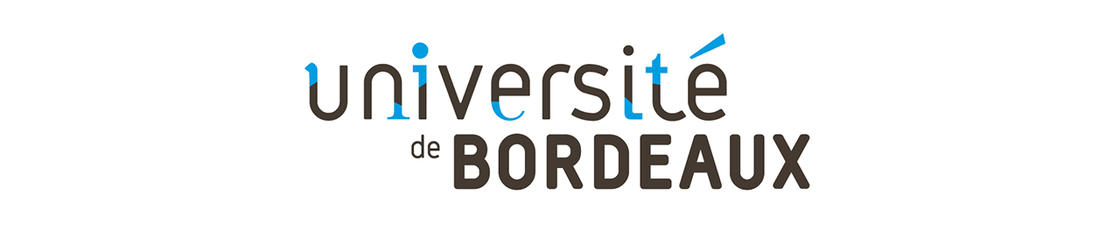
\includegraphics[scale=0.30]{universite-Bordeaux.jpg}~\\[1.5cm]
		\textsc{\LARGE Master 1 Informatique}\\[2cm]
		
		\textsc{\Large Projet de Programmation - Mémoire}\\[1.5cm]
		
		% Titre
		\HRule \\[0.4cm]
		{  \huge{\bfseries Simulation d'écoulement de billes}\\[0.4cm] }
		\HRule \\[2cm]
		
		% Auteurs
		\textsc{GIOVANNANGELI Loann, MAYOLINI Maxime, MOUHOUB Noureddine, RIOU Maxence}\\[0.4cm]
		
		% Bas de page
    	\textsc{\large 5 Avril 2018} \\
        \vspace{2cm}
        \textsc{Lien du dépôt : https://services.emi.u-bordeaux.fr/projet/git/pdp-billes/}
	\end{center}
	\end{titlepage}
    
    
%%% PARTIE 0 : RÉSUMÉ %%%
\section*{Résumé}

L'objectif de notre projet est de réaliser un simulateur 2D d'écoulement de billes. Il doit être capable de simuler un plateau inclinable, sur lequel il est possible d’ajouter des obstacles en forme de lignes droites et des billes. Son interface graphique doit permettre de pouvoir créer, modifier, paramétrer, exporter, importer et lancer la simulation sur un circuit (l’ensemble plateau-billes-obstacles). Le logiciel doit être muni de son propre moteur physique, gérant l’ensemble des collisions du circuit. \\

Le logiciel réalisé va donc permettre de créer son propre circuit, en choisissant ses dimensions et son inclinaison. Des obstacles et des billes pourront être placés dessus. Puis, l'exécution pourra être lancée, utilisant notre moteur physique et montrant le parcours des billes et leurs interactions avec les différents obstacles jusqu'à leur position finale. L'exécution peut être stoppée à n’importe quel moment. Les circuits sont également importables et exportables. De plus, un ensemble de tests (unitaires, de profil et de couverture) sont réalisés sur l’ensemble du projet afin de vérifier que tout fonctionne correctement.  \\

\section*{Abstract}

Our project goal is to achieve a 2D ball flow simulator. It must be able to simulate a reclining plate, on which it is possible to add lines obstacles and balls. Its graphic interface must allow the user to create, configure, export, import and start the simulation of a circuit (ensemble plateau-billes-obstacles). The program must be fitted with its own physics engine, handling the whole collisions in the circuit. \\

The implemented software will be able to create its own circuit, choosing its dimension and inclinaison. Obstacles and balls may be placed on. Then, the execution may be started, using our physics engine et showing the course of the balls and their interactions with the different obstacles until their final position. Execution can be stopped at any moment. Circuits can be imported and exported. Furthermore, a tests set (unit testing, profiling, code coverage) are achieved on the whole project in order to check that all is working correctly.


%%% TABLE DES MATIÈRES %%%
\tableofcontents

%%% TABLE DES ILLUSTRATIONS %%%
\listoffigures

%%% PARTIE 1 : INTRODUCTION %%%
\chapter{Introduction}

\section{Généralités sur les moteurs physiques}

Un moteur physique est une bibliothèque qui offre un ensemble de fonctionnalités permettant de simuler la physique du monde réel : gravité, chutes de corps (solides, liquides ou gazeux), collisions, explosions... Les deux composants principaux d’un moteur physique sont un système de simulation physique responsable du mouvement des objets (dû aux forces qui sont appliquées) et un système de détection et gestion des collisions.

\section{Mécanique newtonienne}


La mécanique est la science qui décrit les mouvements des corps. La mécanique newtonienne (aussi appelée mécanique classique) est la branche qu'on utilise la plupart du temps pour décrire les mouvements des corps sur terre. Elle possède cependant des limites : elle n'est plus juste lorsque les vitesses sont proches de celle de la lumière ou que objets sont trop massifs. De même au niveau atomique pour lequel on se redirige vers la mécanique quantique. Les lois de la mécanique newtonienne répondent tout de même à la majorité des cas qu'on rencontre au quotidien et sont donc implémentées dans la plupart des moteurs physiques.

L’attraction gravitationnelle de la Terre qui attire les objets vers son centre peut être considérée comme une constante dans un moteur physique dont les objets sont proches de la Terre. En effet, la variation de distance entre les objets et la Terre est négligeable. On parle alors de pesanteur et son accélération a pour valeur g = 9,81m/$s^2$. \\

On parle de chute libre lorsque les forces autres que celle de la pesanteur sont négligeables. Il faut comprendre que l'accélération de la pesanteur ne dépend pas de la masse de l'objet. Par conséquent, deux objets en chute libre de même poids mais de masses différentes ont la même accélération. \\

L’accélération de la pesanteur étant constante, nous pouvons utiliser les équations de la cinématique du mouvement rectiligne uniformément accéléré  pour calculer le déplacement des objets attirés vers la Terre. \\

\newpage
Les équations principales d’un mouvement rectiligne uniformément accéléré \cite{02} sont données par :

\(a = F_t / m\)

\(v’ = v + a\)

\(x’ = x + v’\)

avec :
\begin{itemize}
\item a : l'accélération de l'objet
\item m : la masse de l’objet
\item \(F_t\) : la force totale (la somme des forces)
\item v : la vitesse à l’instant actuel
\item v’ : la vitesse à l’instant prochain
\item x : la position courante
\item x' : la prochaine position
\end{itemize}

\section{Collisions}

La force d’un moteur physique est sa capacité à réagir aux événements successifs qui se produisent dans une simulation, en particulier les collisions entre les différents corps. Pour cela, il a besoin de prendre en compte les concepts généraux de la mécanique des collisions, notamment les deux principaux chocs : élastique et inélastique. \\

Lorsque deux billes entrent en collision, il s’agit d’un choc élastique entre deux corps rigides. Pour que le moteur physique réponde bien lorsque deux billes entrent en collision, il doit prendre en compte leur masse et leur vitesse. \\

Il existe des principes généraux \cite{02} qui interviennent lors d’un choc élastique.

\paragraph*{Conservation de la quantité de mouvement}

La somme des quantités de mouvement de chaque corps est conservée avant et après la collision. Dans le cas où le système impose des forces extérieures, cette loi ne sera pas respectée.
La loi de conservation de quantité de mouvement est donnée par :

\(M_1V_{f_1} = M_1V_{i_1} + P\)

\(M_2V_{f_2} = M_2V_{i_2} - P\)

Ce qui donne :

\(M_1V_{f_1} + M_2V_{f_2} = M_1V_{i_1}+M_2V_{i_2}\)

\(M_x\) est la masse de l’objet \(x\).
\(V_{i_x}\) est la vitesse initiale de l’objet \(x\).
\(V_{f_x}\) est la vitesse finale de l’objet \(x\).
\(P\) est le vecteur de percussion du choc (variation de la quantité de mouvement en négligeant les autres forces).

\paragraph*{Conservation de l'énergie cinétique}

La somme de l’énergie cinétique des deux objets est la même avant et après la collision. Cette loi n'est pas respectée lors d'un choc inélastique.
La loi de conservation de l'énergie cinétique est donnée par :

\(M_1V_{i_2} + M_2V_{i_2} = M_1V_{f_2} + M_2V_{f_2}\)

où \(M_x\) est la masse de l’objet \(x\), et \(V_i\) (resp. \(V_f\)) est la vitesse initiale (resp. finale).

\newpage
\section{Limites des moteurs physiques}

Avoir un comportement le plus réaliste possible est bien évidemment l’objectif majeur d’un moteur physique. Cependant, il est impossible d'en concevoir un qui puisse reproduire la physique sur terre avec exactitude. \\

Une des premières limites à laquelle on peut penser est la précision des nombres représentant les forces ou la position des objets. Si cette précision est trop basse, le comportement des objets ne sera pas satisfaisant et les données de la simulation ne seront pas exploitables. Plus la précision est importante, plus la simulation sera réaliste. Cependant, cette précision est coûteuse en puissance de calcul, en temps et en mémoire. \\

On peut également penser aux phénomènes dits aléatoires ou imprédictibles (théorie du chaos) qui interviennent et qui font que la simulation d’une expérience est différente du déroulement de cette expérience dans la réalité.

%%% PARTIE 2 : ANALYSE DE L'EXISTANT %%%
\chapter{Analyse de l'existant}

\section{Moteur physique}

\subsection{Quelques moteurs 3D}

\subsubsection{PhysX}

Unity est un moteur de jeu multi-plateformes très répandu pour la conception d’applications graphiques 3D. Il intègre le moteur physique PhysX qui permet une simulation en temps réel très réaliste. \\

PhysX est à l’origine conçu par la société AGEIA en 2005. Au même moment, AGEIA développe également le premier processeur physique (Physics Processing Unit) dédié pour jeux vidéos PC. Ce processeur porte également le nom PhysX et a pour but de gérer les calculs de simulation de la physique des jeux vidéo utilisant le moteur physique PhysX (on parle d’accélération matérielle). En 2008, NVIDIA rachète AGEIA et la production des processeurs PhysX est stoppée. Cependant, le moteur physique est récupéré et l’accélération matérielle est désormais réalisée par les GPU (cartes graphiques) NVIDIA. Le SDK (kit de développement logiciel) de PhysX est rendu public et gratuit et est rapidement supporté par la plupart des marques de GPU. Aujourd’hui, l’accélération matérielle NVIDIA PhysX est supportée par de nombreux jeux, mais elle est également utilisée dans la recherche et l’enseignement. \\

	Unity, quant à lui, est très facile d’utilisation : grâce à une interface simple, on peut créer un plan de taille modulable, l’incliner, poser des billes et des obstacles sur ce plan et lancer une simulation.

    
\subsubsection{Havok}

Le concurrent de PhysX est le moteur physique Havok, qui est également utilisé par de nombreux jeux vidéo PC ou consoles. Anciennement détenu par Intel, Microsoft en est le propriétaire depuis 2015. Pendant des années, seul le processeur (CPU) était sollicité pour les calculs. Ce n’est que depuis récemment qu’il bénéficie de l’accélération matérielle GPU. Autrefois accessible gratuitement sur internet, le SDK Havok est désormais payant depuis son rachat par Microsoft.

\subsubsection{Bullet}

Bullet est une bibliothèque qui regroupe un ensemble de fonctionnalités qui permet de simuler l'interaction entre des objets de différents types (sphère, cylindre,  rectangle, etc). Il offre un modèle des corps absolument rigide négligeant toute déformation. Bullet a été retranscrit dans plusieurs langages de programmation, et notamment en Java sous le nom JBullet. Il est utilisé, par exemple, dans les jeux vidéo “Asphalt” et “Fast and Furious”.

\subsection{Quelques moteurs 2D}

Box2D est un moteur physique 2D open-source développé en C++. Il est également utilisé dans de nombreux jeux 2D, et notamment dans le célèbre jeu mobile “Angry Birds”. Très complet, il détecte et gère les collisions entre des corps rigides de nombreuses formes, les frottements ou encore l’élasticité. Il a été porté sur d’autres langages de programmation, comme Java sous le nom de JBox2D. \\

Chipmunk est un moteur physique 2D en temps réel disponible en deux versions : une gratuite et l’autre professionnelle. Il dispose d’un système de détection de collisions flexible, de telle sorte qu’il permet à l'utilisateur de paramétrer les forces et coefficients en jeu selon le type de collision. Il est également disponible sur toutes les plateformes. \\

Le problème principal est que ces moteurs physiques sont trop complets par rapport à nos besoins. Par conséquent, les utiliser rendrait notre programme trop lourd.

\section{Algorithmes}

\subsection{Algorithme général}

L'algorithme général d’un simulateur de physique discrète synchrone, relié à un pas de temps, est basé sur les étapes suivantes :
\begin{itemize}
\item Calculer les nouvelles positions de chaque objet sans prendre en considération les collisions.
\item Détecter les collisions selon le type des corps concernés.
\item Traiter les collisions : calcul des nouvelles vitesses.
\item Mettre à jour l’état des objets concernés par l’étape précédente.
\item Reprendre les étapes jusqu’à la fin de la simulation.
\end{itemize}

\begin{figure}[H]
\centering
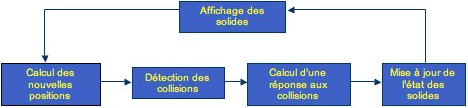
\includegraphics[scale=1.0]{algo_general.PNG}
\caption{Schéma de l'algorithme général \cite{03}}
\end{figure}

\subsection{Détection de collisions}

\subsubsection{Définition d'une collision}

Une collision est un choc entre deux objets. La détection des collisions nécessite plusieurs algorithmes selon la forme des objets présents dans le moteur physique. En effet, la manière de détecter une collision entre deux cercles est différente de celle d’une collision entre un cercle et une droite ou un rectangle. \\

La détection d’une collision entre deux cercles est très simple. On récupère les coordonnées des deux centres et on calcule la distance qui les sépare. Si cette distance est inférieure à la somme des rayons, alors il y a collision. \\

\newpage
L’algorithme de détection d’une collision entre un cercle et un segment est un peu plus complexe. Cela se fait par étapes. Il faut d’abord vérifier si le cercle est en collision avec la droite passant par ce segment. Si ce n’est pas le cas, il n’y a pas collision. Si c’est le cas, on calcule le point de projection perpendiculaire au centre de la bille sur la droite. Si ce point est sur le segment, alors il y a collision. Si ce n’est pas le cas, on vérifie si les points d’extrémité du segment sont à l’intérieur du cercle pour savoir s’il y a collision ou non. Ci-dessous se trouve un schéma explicatif.

\begin{figure}[H]
\centering
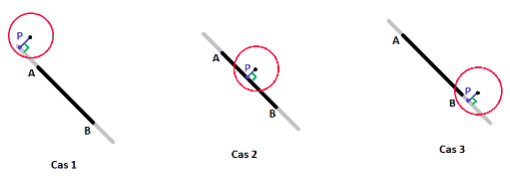
\includegraphics[scale=1.0]{detect_collision.PNG}
\caption{Schéma des différents cas de détection de collisions}
\end{figure}

Cas 1 : le cercle est en collision avec la droite, alors on calcule la projection P. Ce point n’est pas sur le segment AB et A et B ne sont pas dans le cercle, donc il n’y a pas collision. \\

Cas 2 : le cercle est en collision avec la droite, alors on calcule la projection P. Ce point est sur le segment AB, alors il y a collision. \\

Cas 3 : le cercle est en collision avec la droite, alors on calcule P. Ce point n’est pas sur le segment AB mais B est dans le cercle (distance au centre inférieure au rayon), donc il y a collision.

\subsubsection{Optimisations}

L’algorithme trivial de détection des collisions consiste à prendre chaque objet un à un et vérifier s’il est en collision avec chaque objet. La complexité en temps de cet algorithme est quadratique (O($n^2$), n étant le nombre d’objets). Il est donc coûteux en terme de calculs. Heureusement, il existe une technique simple pour diminuer drastiquement cette complexité : il suffit de partitionner l’espace. De cette manière, un objet appartient à une portion de l’espace et vérifie uniquement la collision avec ses voisins, c’est-à-dire les objets qui se situent dans la même portion d’espace. En effet, il est inutile de vérifier la collision d’un objet avec un autre objet se situant à une très grande distance, puisqu’on est certain qu’il n’y a pas collision.

Il existe plusieurs méthodes de partitionnement de l’espace \cite{06} qui diffèrent selon leur complexité de mise en œuvre et leurs performances (diminution du nombre de calculs). Il est difficile d’en déclarer une meilleure que les autres, elles ont chacune des avantages et inconvénients selon les cas d’utilisation.

\newpage
\paragraph{Grille}

D’un point de vue algorithmique, c’est la méthode la plus simple à mettre en œuvre.
Le principe est de diviser l’espace en une grille de cellules de taille identique. Cependant, la taille des cellules pose problème et doit être réfléchie. Si elles sont trop grandes, il se peut qu’il y ait beaucoup d’objets dans une même cellule, et donc le nombre de calculs reste important. Si elles sont trop petites, on se retrouve avec un nombre très élevé de cellules à stocker, ce qui est coûteux en mémoire. De plus, si les objets sont surtout localisés dans une partie de l’espace, on stocke un grand nombre de cases vides inutilement. Cette méthode présente donc des limites et n’est pas la meilleure en terme de gain de performances. \\

Ci-dessous se trouve un exemple de grille.

\begin{figure}[H]
\centering
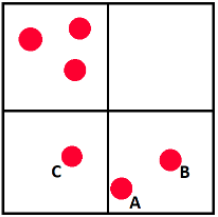
\includegraphics[scale=0.6]{grid.PNG}
\caption{Schéma d'une grille}
\end{figure}

L’objet A se situe dans la même cellule que l’objet B : il va donc devoir vérifier la collision avec lui.

\paragraph{QuadTree}

Le quadtree (arbre quaternaire) est la méthode la plus utilisée pour partitionner un espace 2D. On part d’un nœud racine qui représente l’ensemble de l’espace. Ce nœud possède 4 nœuds fils représentant chacun une partie de l’espace (4 quadrants de taille égale). Le principe est simple : lorsqu’un nœud contient un certain nombre d’objets, il se divise à nouveau en 4 sous-quadrants. Cet algorithme est récursif. On peut donc penser à une sorte de grille dynamique, mais il a un gros avantage : on subdivise uniquement les cellules contenant beaucoup d’objets, par conséquent on ne stocke pas un grand nombre de cellules vides comme c’est le cas pour la grille. L’inconvénient de cette méthode est qu’elle peut entraîner un arbre déséquilibré selon la répartition des objets. \\

Ci-dessous se trouve un exemple de Quadtree.

\begin{figure}[H]
\centering
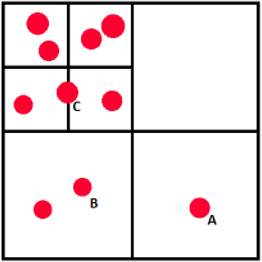
\includegraphics[scale=0.6]{quadtree.PNG}
\caption{Schéma d'un Quadtree}
\end{figure}

L’objet A est seul dans sa région : il n’a donc pas besoin de vérifier de collisions. L’objet B vérifie la collision avec le seul autre objet dans sa région. Enfin, l’objet C ne rentre pas complètement dans une sous-région. Il vérifie donc la collision avec sa région parente, c’est-à-dire tous les objets du quadrant supérieur gauche.

\begin{figure}[H]
\centering
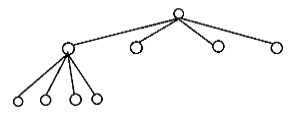
\includegraphics[scale=0.6]{arbre_quadtree.PNG}
\caption{Arbre d'un Quadtree}
\end{figure}

Ce quadtree représente le découpage des régions du cas ci-dessus. Le nœud racine représente l’ensemble de l’espace. On peut voir que le quadrant supérieur gauche est divisé en 4 sous-régions car il contenait trop d’objets. \\

La même méthode récursive de partitionnement est utilisée pour les espaces 3D avec des octrees (un nœud possède 8 fils).

\paragraph{K-d tree}

Un k-dimensions tree est un arbre binaire utilisé pour le partitionnement de l’espace à k dimensions. Dans un espace 2D, le principe est de diviser alternativement l’espace en X et en Y selon la médiane des coordonnées X et la médiane des coordonnées Y des objets d’une région, jusqu’à ce que tous les objets soient séparés. Cette méthode a l’avantage de produire un arbre équilibré. \\

Ci-dessous se trouve un exemple de k-d tree.

\begin{figure}[H]
\centering
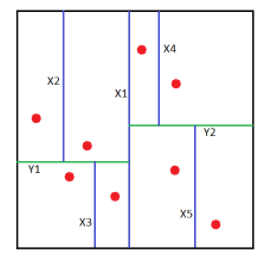
\includegraphics[scale=0.6]{kdtree.png}
\caption{Schéma d'un k-d tree}
\end{figure}

\begin{figure}[H]
\centering
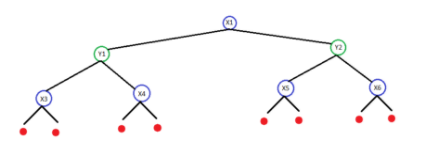
\includegraphics[scale=0.6]{arbre_kdtree.png}
\caption{Arbre d'un k-d tree}
\end{figure}

La ligne X1 découpe l’espace en 2 sous-régions grâce à la médiane des coordonnées X des points. Ensuite, on découpe à nouveau chacune de ces sous-régions grâce à la médiane des coordonnées Y des points. Enfin, on finit par une découpe en X : tous les points sont séparés et l’algorithme s’arrête.

\newpage
\subsection{Résolution de collisions}

Il existe de nombreux algorithmes pour gérer les collisions entre les différents corps dans une simulation.

\subsubsection{Collision entre deux billes}

\begin{figure}[H]
\centering
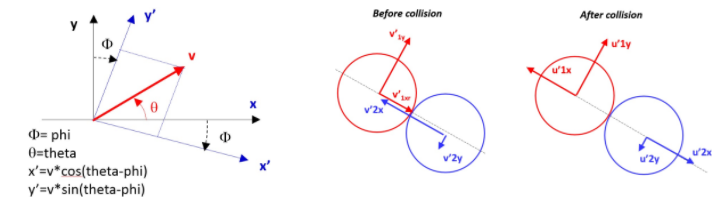
\includegraphics[scale=0.9]{collision_bille_bille.png}
\caption{Schéma d'une collision entre deux billes \cite{04}}
\end{figure}

La gestion de ce type de collision dépend de la vitesse, de l’angle d’arrivée de chaque bille et de l’angle de collision qui est le segment reliant les deux centres. \\

L’algorithme s'appuie sur les équations des vitesses obtenues par les deux lois de conservation de quantité de mouvement et de l’énergie cinétique d’un choc élastique, de telle sorte que les nouvelles vitesses X dans notre nouveau système de coordonnées suivent le même résultat que la collision 1D \cite{02}, et les composantes Y ne changent pas. \\

\newpage

Cela implique que :

\[u’_1x = ((m_1-m_2)*v’_1x+(m_2+m_2)*v’_2x)/(m_1+m_2)\]
\[u’_1y = v’_1y\] \\

Or, d'après le schéma, on a :

\[v’_1x = v_1*cos(direction1-\phi)\]
\[v’_1y = v_1*sin(direction1-\phi)\] \\

Donc l'équation de la nouvelle vitesse sera de la forme :

\[V_x = u_x’ cos(\phi) - u_y’ sin(\phi)\]
\[V_y = u_x’ sin(\phi) + u_y’ cos(\phi)\]

Où :

\begin{itemize}
\item \(\phi\) est l'angle de collision.
\item "direction" est la direction de la bille 1.
\item \(v_i\) est la vitesse de la bille i.
\end{itemize}


\begin{algorithm}[h]
\KwIn{Ball1, Ball2}
    \caption{{\bf CollisionBallBall} \label{CollisionBallBall}}
   \nl {\bf direction1} \(\leftarrow\) Ball1.getAngle();\\
   \nl {\bf direction2} \(\leftarrow\) Ball2.getAngle();\\
   \nl {\bf collisionAngle} \(\leftarrow\) getCollisionAngle();\\
   \nl {\bf newV1x} \(\leftarrow\) V1 * Cos(direction1-collisionAngle);\\ 
   \nl {\bf newV1y} \(\leftarrow\) V1 * Sin(direction1-collisionAngle);\\
   \nl {\bf newV2x} \(\leftarrow\) V2 * Cos(direction2-collisionAngle);\\ 
   \nl {\bf newV2y} \(\leftarrow\) V2 * Sin(direction2-collisionAngle);\\
   \nl {\bf finalV1x} \(\leftarrow\) ((mass1-mass2) * newV1x + (2*mass2) * newV2x)/(mass1+mass2);\\ 
   \nl {\bf finalV2x} \(\leftarrow\) ((2*mass1) * newV1x + (mass2 - mass1) * newV2x)/(mass1+mass2);\\
   \nl {\bf Ball1.Vx} \(\leftarrow\) Cos(collisionAngle) * finalV1x - Sin(collisionAngle) * newV1y;\\
   \nl {\bf Ball1.Vy} \(\leftarrow\) Sin(collisionAngle) * finalV1x + Cos(collisionAngle) * newV1y;\\
   \nl {\bf Ball2.Vx} \(\leftarrow\) Cos(collisionAngle) * finalV2x - Sin(collisionAngle) * newV2y;\\
   \nl {\bf Ball2.Vy} \(\leftarrow\) Sin(collisionAngle) * finalV2x + Cos(collisionAngle) * newV2y;
\end{algorithm}

\clearpage

\subsubsection{Collision entre bille et obstacle}

\begin{figure}[H]
\centering
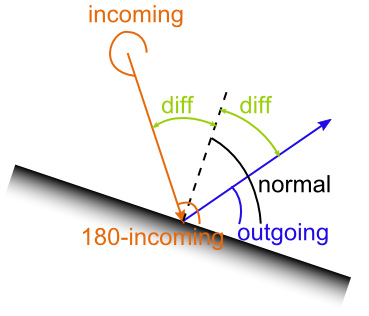
\includegraphics[scale=1]{collision_bille_obstacle.png}
\caption{Schéma d'une collision entre une bille et un obstacle. \cite{05}}
\end{figure}

Ce type de collision est très répandu dans les jeux de billard et de flipper, dans lesquels une bille entre en collision avec un mur horizontal ou vertical. Ces derniers sont les cas basiques du problème général de rebondissement contre un obstacle : il s’agit d’inverser la composante vitesse sur la normale à la surface percutée. \\

Le principe de base de cette collision est la réflexion de l’angle d’arrivée de la bille, c’est-à-dire que l’angle d’arrivée est le même pour la sortie. \\

D’après la figure, l’angle de rebond est la soustraction entre l’angle de la normale et l’angle de la différence. En revanche, la différence est obtenue par l’angle d’arrivée et l’angle de la normale. En remplaçant l’angle de la différence par sa valeur, on obtient l’angle de sortie en fonction de la normale et de l’angle d’arrivée.

\begin{algorithm}[h]
\KwIn{Ball, Obstacle}
    \caption{{\bf CollisionBallObstacle} \label{CollisionBallObstacle}}
   \nl {\bf incoming} \(\leftarrow\) Ball.getAngle();\\
   \nl {\bf normal} \(\leftarrow\) getNormaleAngle();\\
   \nl {\bf outgoing} \(\leftarrow\) 2 * normal -180 - incoming;\\
   \nl {\bf Ball.Vx} \(\leftarrow\) Cos(outgoing) * Ball.getSpeed();\\
   \nl {\bf Ball.Vy} \(\leftarrow\) Sin(outgoing) * Ball.getSpeed();\\
\end{algorithm}


%%% PARTIE 3 : ANALYSE DES BESOINS %%%
\chapter{Analyse des besoins}

\textit{Dans cette partie, une note de priorité est associée à chaque besoin. Elle va de 1 à 4 : 1 pour un besoin anecdotique, 4 pour un besoin absolument nécessaire.}

\section{Besoins fonctionnels}

\subsection{Moteur physique}

L’écoulement des billes dans le circuit doit être simulé par un moteur physique en 2D. On utilisera des combinaisons linéaires pour représenter les déplacements. Pour être réaliste, notre moteur physique doit respecter les lois de la physique terrestre. \\

Notre programme doit gérer le déplacement des billes en prenant en compte la gravité, ainsi que les collisions entre tous les objets du circuit (bille-bille, bille-obstacle). Pour cela nous devons nous baser sur la mécanique du point, notamment le mouvement rectiligne uniformément accéléré. Pour les collisions entre billes, nous devons utiliser les équations du choc élastique. 


\subsubsection{Structure des objets}

Dans le circuit, on distingue deux types d’objets : les billes et les obstacles.


\paragraph{Billes - Priorité : 4}

Le déplacement d’une bille nécessite de connaître sa position ainsi que sa vitesse pour calculer sa prochaine position. Sa vitesse est calculée en fonction de l’accélération engendrée par la gravité. La position et le rayon vont servir pour la détection des collisions. Lors d’un choc entre billes, nous devons connaître leur masse et leur vitesse respectives pour répondre aux lois de conservation de la quantité de mouvement et de conservation de l’énergie cinétique (choc élastique). Les billes doivent donc posséder une position, un rayon, une masse et une vitesse dans une certaine direction.

\paragraph{Obstacles - Priorité : 4}

Les obstacles sont des segments et sont infranchissables, les billes doivent s'y heurter. Pour détecter les collisions entre billes et obstacles on doit connaître la position des extrémités du segment. Ces collisions sont des chocs inélastiques, l’énergie cinétique de la bille doit diminuer, ainsi que sa vitesse. Il faut donc utiliser un coefficient de restitution inférieur à 1.

\newpage
\subsubsection{Forces en jeu}

Un moteur physique réaliste prend en compte plusieurs forces : force de gravité, force de réaction (normale) et forces de frottements (air et cinétique). Ces forces sont nécessaires pour le calcul du vecteur vitesse de la bille.

\paragraph{Force de gravité - Priorité : 4}

La gravité a un impact sur le déplacement des billes, elle les attire vers le bas. La force de gravité est constante : 9,81N. Cette constante est présente dans le calcul de l’accélération de la bille. La force de la gravité sera atténuée par l’inclinaison du plan (voir paragraphe suivant, “Force de réaction”). 

\paragraph{Force de réaction - Priorité : 4}

La force de réaction du plan (circuit) influence l’accélération des billes. Plus le plan est vertical (inclinaison proche de 90 degrés), plus la force réaction du plan est faible et donc l’accélération est élevée. Lorsque l’inclinaison est égale à 90 degrés, la force de réaction du plan est nulle et l’accélération est égale à la force de la gravité. A l’inverse, si l’inclinaison est de 0 degré, le plan est horizontal et la force de réaction du plan s’oppose parfaitement à la gravité, donc aucune bille ne doit bouger. \\

La force de réaction d’un obstacle est de même direction que sa normale, et cette dernière doit être utilisée pour calculer l’angle de rebond lors d’une collision bille-obstacle. 


\paragraph{Force de frottements - Priorité : 2}

Une physique réaliste sur terre comporte des frottements, ce qui a pour effet de ralentir et faire rouler les billes.  Le moteur physique doit donc prendre en compte les frottements de l’air et de la surface (potentiellement différents en fonction du matériau du circuit et des obstacles).

\subsection{Gestion du circuit}

\subsubsection{Billes - Priorité : 4}

Un circuit doit contenir une liste de billes et permettre l’ajout ou la suppression d’une bille. L’ajout d’une bille ne peut pas se faire si elle va être ajoutée par-dessus un objet déjà existant.

Pour vérifier qu’une bille a bien été ajoutée au circuit, on vérifie qu’elle est bien présente dans la liste de billes du circuit. Il faut aussi vérifier que l’ajout d’une bille est bien refusé si celle-ci est censée être ajoutée par-dessus un objet déjà existant. Pour cela, on ajoute un objet dans le circuit puis on essaie d’ajouter une bille aux mêmes coordonnées que l’objet précédent. La liste de billes du circuit ne doit alors pas contenir la bille en question.

\subsubsection{Traces des billes - Priorité : 4}

Chaque bille du circuit doit contenir une liste de points correspondant à sa trace : ses positions précédentes lors d’une exécution. Cette trace doit être visualisable en temps réel au cours d’une exécution afin de suivre le déplacement des billes.


\subsubsection{Obstacles - Priorité : 4}

Un circuit doit contenir une liste d’obstacles et permettre l’ajout ou la suppression d’un obstacle. Un obstacle ne doit pas pouvoir être placé par-dessus une bille déjà existante dans le circuit. Par contre, il doit être possible de pouvoir le placer en croisant un autre obstacle.

Pour vérifier qu’un obstacle a bien été ajouté au circuit, on vérifie qu’il est bien présent dans la liste d’obstacles du circuit. Il faut aussi vérifier que l’ajout d’un obstacle est bien refusé si celui-ci est censé être ajouté par-dessus une bille déjà existante. Pour cela, on ajoute une bille dans le circuit puis on essaie d’ajouter un obstacle dont la droite passe par les coordonnées de la bille. La liste d’obstacles du circuit ne doit alors pas contenir l’obstacle en question.


\subsubsection{Réinitialisation - Priorité : 3}

L’application doit proposer un moyen de suppression de toutes les billes, tous les obstacles ou tous les objets (billes et obstacles).

Pour vérifier que la réinitialisation a fonctionné, on vérifie le contenu des listes d’objets (bille, obstacle ou les deux) qui ont été supprimés.


\subsubsection{Redimensionnement - Priorité : 3}

L’application doit permettre de modifier la longueur et la largeur du circuit. Si la taille du circuit est réduite, les objets passant hors du circuit doivent être supprimés.

Pour tester que le redimensionnement a fonctionné comme prévu, on vérifie que les nouvelles dimensions du circuit correspondent bien à celles entrées, et on parcourt ses listes de billes et d’obstacles (préalablement remplies) en vérifiant qu’aucun objet ne soit hors du circuit.


\subsubsection{Inclinaison - Priorité : 4}

L’inclinaison du circuit doit être comprise entre 0 degré et 90 degrés. Elle n’agit que sur un seul axe du circuit. Elle doit pouvoir être modifiée en toutes circonstances (que la simulation soit en cours ou non).

\subsubsection{Optionnel - Fusion de circuits}

L’application permet de fusionner deux circuits, c’est-à-dire les “coller” l’un à côté de l’autre de façon horizontale ou verticale. Les deux circuits à fusionner doivent avoir la même dimension sur le côté où ils sont fusionnés.

\subsection{Interface graphique}

Afin de permettre une utilisation plus simple et dynamique de l’application, celle-ci devra être utilisable au travers d’une interface graphique.

\subsubsection{Affichage du circuit - Priorité : 4}

L’interface graphique doit permettre de visualiser l’état du circuit durant toute l’exécution du programme (phase de création de circuit ou phase de simulation d’écoulement de billes).

\subsubsection{Paramétrage du circuit - Priorité : 3}

L’interface doit permettre de paramétrer le circuit, c’est-à-dire de pouvoir le modifier selon les exigences demandées dans la gestion du circuit, le tout via la souris ou différents boutons.

\subsubsection{Optionnel - Zoom}

L’interface graphique est zoomable : l’utilisateur peut choisir d’agrandir visuellement une zone du circuit afin de mieux observer son contenu.

\subsubsection{Optionnel - Paramétrer le coefficient de restitution des obstacles}

L’interface graphique permet de demander la modification du coefficient de restitution d’un obstacle.

\subsection{Gestion de l'exécution}

\subsubsection{Démarrer une simulation - Priorité : 4}

L’application doit permettre de démarrer la simulation d’écoulement des billes. À ce moment, l’utilisateur ne doit plus pouvoir ajouter d’objets au circuit ni le modifier, et les billes doivent être soumises aux différentes forces du moteur physique.

\subsubsection{Mettre en pause une simulation - Priorité : 2}

L’application doit permettre de mettre en pause une simulation. Les billes ne doivent donc plus bouger, et l’utilisateur peut à nouveau utiliser les fonctionnalités de paramétrage et de création d’objets.

\subsubsection{Optionnel - Modifier la vitesse de la simulation}

L’application permet de changer la vitesse d’exécution de la simulation. En outre, on doit avoir l’impression que les billes accélèrent ou décélèrent en fonction de ce facteur.

\subsection{Gestion des fichiers}

\subsubsection{Export - Priorité : 3}

L’application doit permettre de sauvegarder les informations essentielles d’un circuit. On doit donc, a minima, sauvegarder les données du circuit, de chaque obstacle et de chaque bille (avec sa trace).

\subsubsection{Import - Priorité : 3}

L’application doit permettre de lire un fichier de sauvegarde de circuit et le recréer avec tous ses paramètres : ses dimensions, son inclinaison, ses billes et ses obstacles. \\

Pour vérifier l’import et l’export, on crée un circuit en mémoire dont on sauvegarde les données et on l’exporte dans un fichier puis on l’importe. Si le circuit résultant de l’import possède les mêmes données que le premier, c’est que l’opération d’export/import a bien sauvegardé et rechargé les données du circuit.

\subsubsection{Optionnel - Vidéo de l'exécution}

L’application propose d’enregistrer une simulation puis d’exporter cet enregistrement sous la forme d’un fichier vidéo.

\subsubsection{Optionnel - Impression du circuit}

L’application permet d’imprimer un circuit. L’impression ne prend pas en compte les traces de billes (s’il y en a). Le but est d’avoir une version physique du circuit qui permettrait de reproduire les expériences dans la réalité.

\newpage

\section{Besoins non-fonctionnels}

\subsection{Performances}

\subsubsection{Temps de chargement - Priorité : 2}

Le temps de chargement est le temps que doit attendre l’utilisateur après chaque interaction avec l’interface graphique.

Afin que l’utilisation de l’application soit agréable, ce temps est fixé à titre indicatif à deux secondes.

Pour vérifier que les interactions avec l’interface graphique aient la durée escomptée, on fait un test qui vérifie que la durée de la ou des fonctions mises en œuvre par l’interaction soit inférieure à deux secondes.


\subsubsection{Fluidité de la simulation - Priorité : 3}

La simulation doit être visuellement réaliste : les billes doivent donner l’impression de glisser et non pas de se téléporter à chaque déplacement.

\subsection{Robustesse du moteur physique - Priorité : 4}

Il est important que le moteur physique fonctionne correctement afin de garantir le bon comportement des billes. Les tests doivent donc être accentués dessus (plus nombreux et plus robustes).

\subsection{Portabilité - Priorité : 3}

Afin que l'application soit utilisable par tout utilisateur, l’application doit être multi-plateformes et être exécutable sous Windows, Linux et MacOS.

\subsection{Ergonomie - Priorité : 1}

L’utilisateur doit pouvoir interagir facilement et rapidement avec les fonctionnalités proposées par l’interface graphique.



%%% PARTIE 4 : DESCRIPTION DU LOGICIEL %%%
\chapter{Description du logiciel}

\section{Utilisation}

\subsection{Installation}

L'application a été développée en Java 8. Comme bibliothèque importante, on notera l'utilisation de la dernière version de Java SWING. Nous sommes conscients que SWING a été délaissé il y a maintenant plusieurs années au profit de JavaFX, cependant nous avions déjà les connaissances nécessaires pour réaliser notre interface sous SWING (mais pas sous JavaFX). Nous avons donc préféré utiliser la bibliothèque SWING, bien que moins récente et sans doute moins adaptée, afin d'accélérer la partie développement de l'interface et privilégier ainsi le développement du moteur physique.

Les tests ont été réalisés avec la bibliothèque JUnit 4.

\paragraph*{Exécutable} L'application étant réalisée en java, l'exécutable devrait pouvoir marcher sur n'importe quelle machine possédant un JRE (Java Runtime Environment) ou JDK (Java Development Kit) de version 8 ou plus.

\paragraph*{Compilation} Pour exécuter l'application en recompilant les fichiers, il faut au minimum un JDK 8. Ensuite, il y a deux solutions :
\begin{itemize}
\item via un IDE : le projet a été réalisé sous Eclipse (Neon ou plus). Il doit aussi être possible d'importer le projet sous IntelliJ 11.
\item via un terminal : se placer dans le dossier src. Pour compiler, faire la commande \texttt{javac \_default/Main.java} ; puis, pour exécuter, effectuer \texttt{java \_default.Main} . La compilation va créer des fichiers ".class" à coté de chaque fichier ".java" du code source. Cette méthode marche sous Windows (testé sous Windows 10) et sous Linux. Vous pouvez retrouver les informations de la compilation par terminal dans le fichier \texttt{README.md}.

\end{itemize}

\newpage
\subsection{Interface homme-machine}

Lors du lancement de l’application, la fenêtre principale s’affiche.

\begin{figure}[H]
\centering
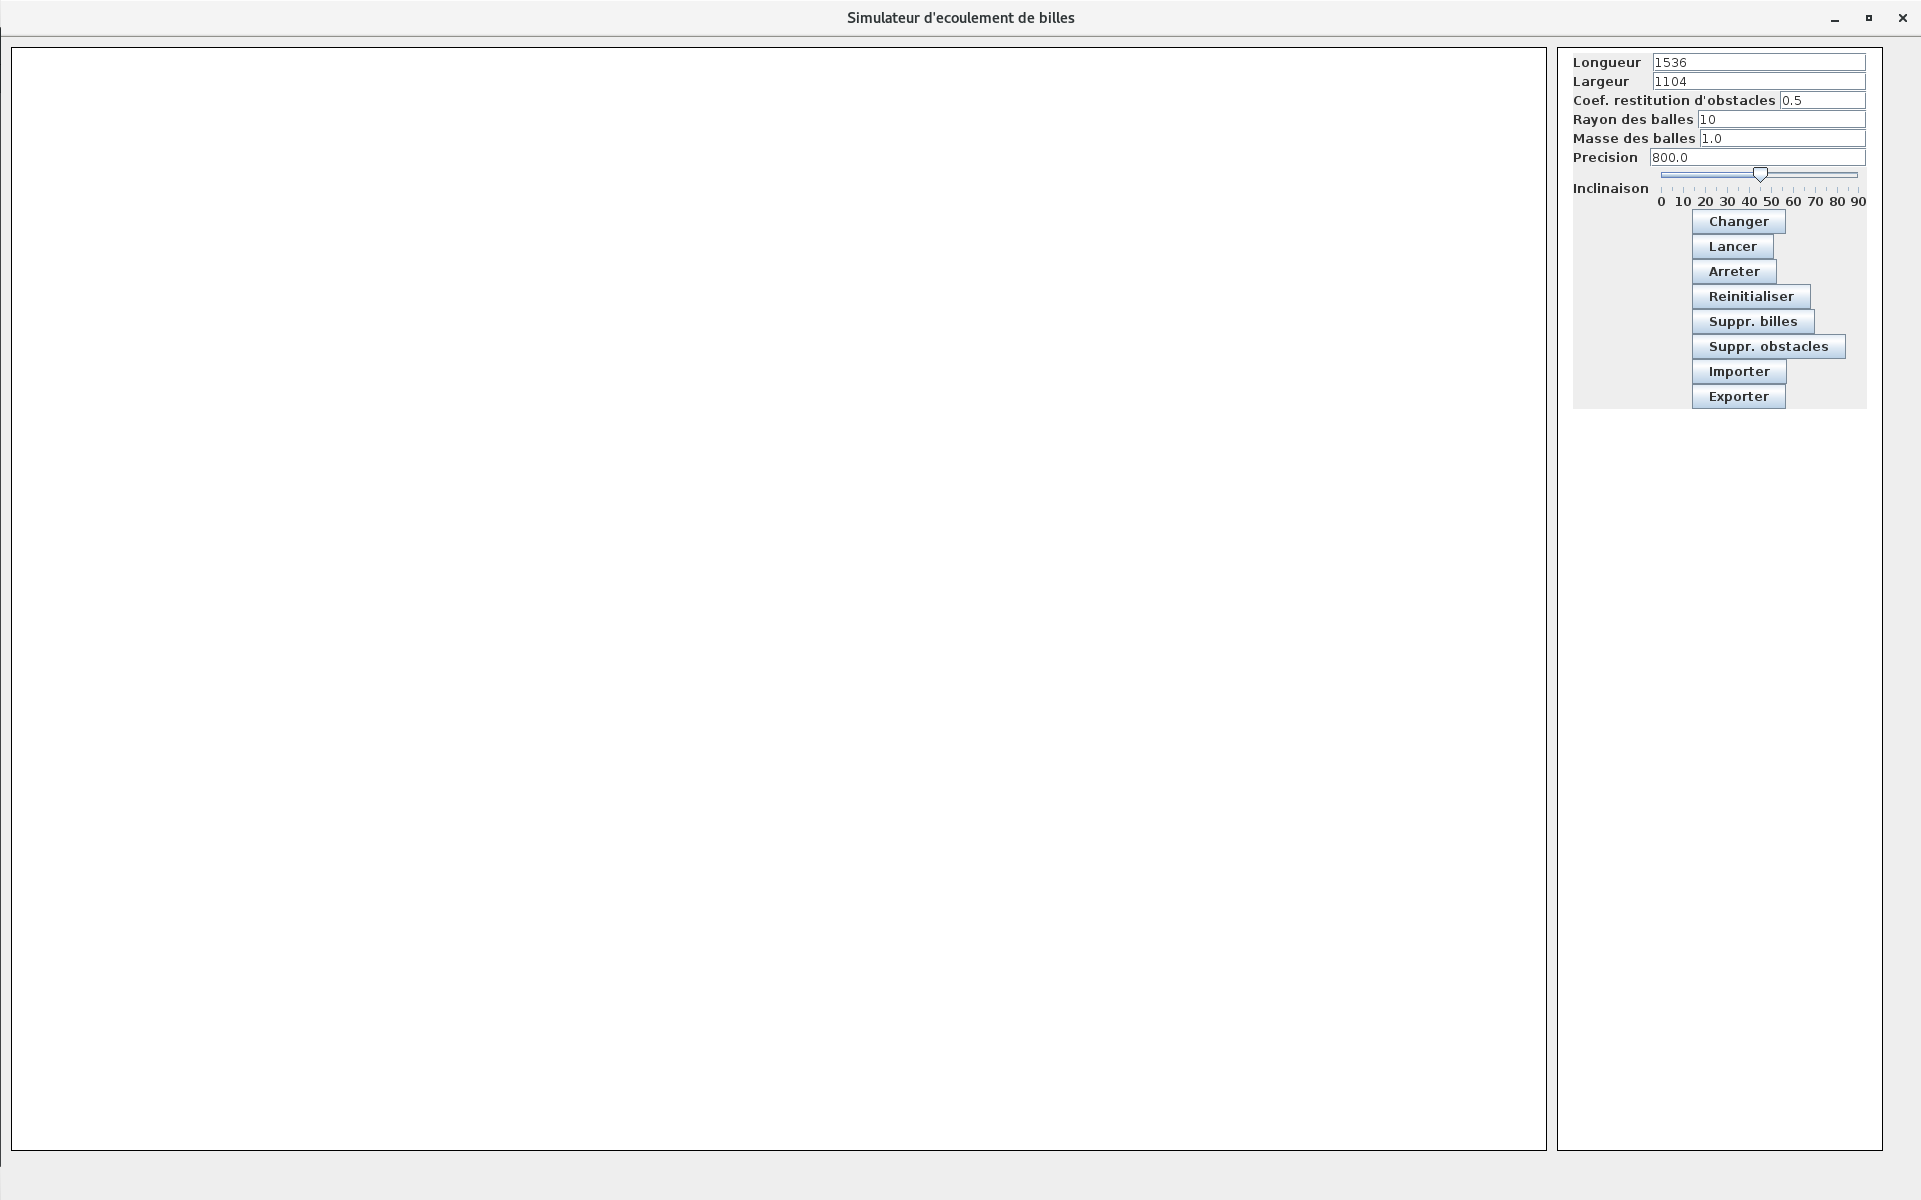
\includegraphics[scale=0.25]{main_frame.png}
\caption{Fenêtre principale de l'application}
\end{figure}

Cette fenêtre est découpée en deux parties :
\begin{itemize}
\item Le grand rectangle blanc de gauche représente le panneau de dessin, sur lequel l’utilisateur peut cliquer pour créer, modifier ou supprimer des billes et des obstacles.
\item Le rectangle plus fin de droite représente le panneau de paramétrage, sur lequel l’utilisateur peut cliquer sur des boutons pour modifier plus globalement le circuit, lancer et stopper la simulation, ainsi qu’importer et exporter un circuit.
\end{itemize}

\newpage
\subsubsection{Panneau de dessin}

Sur le panneau de dessin, l’utilisateur peut interagir avec les objets du circuit. \\

Voici les actions possibles :
\begin{itemize}
\item Créer une bille : l’utilisateur fait un clic droit là où il veut créer une bille (l’endroit où il clique sera le centre de la bille). Il est impossible de créer une bille par-dessus des obstacles ou billes existants.
\item Créer un obstacle : l’utilisateur fait un clic gauche pour commencer à créer un obstacle (l’endroit où il clique sera la première extrémité de l’obstacle), puis le maintient et glisse jusqu’à l’endroit où il souhaite finir l’obstacle (l’endroit où il relâche le clic gauche sera la seconde extrémité de l’obstacle). Lors du glissement, un petit carré noir indique sur l’écran la position de la première extrémité. Il est impossible de créer un obstacle par-dessus des billes existantes, mais il est possible de le faire par-dessus des obstacles. Cela permet à l’utilisateur de pouvoir créer facilement des formes d’obstacles plus complexes.
\item Modifier ou supprimer un objet : l’utilisateur fait un clic droit sur l’objet qu’il souhaite modifier ou supprimer. Une petite fenêtre cliquable s’ouvre alors, qui permet de choisir l’option souhaitée. Si l’utilisateur choisit “Parametres”, une nouvelle fenêtre adaptée à l’objet sélectionné s’ouvre, permettant de modifier ses caractéristiques.
\end{itemize}

\begin{figure}[H]
\centering
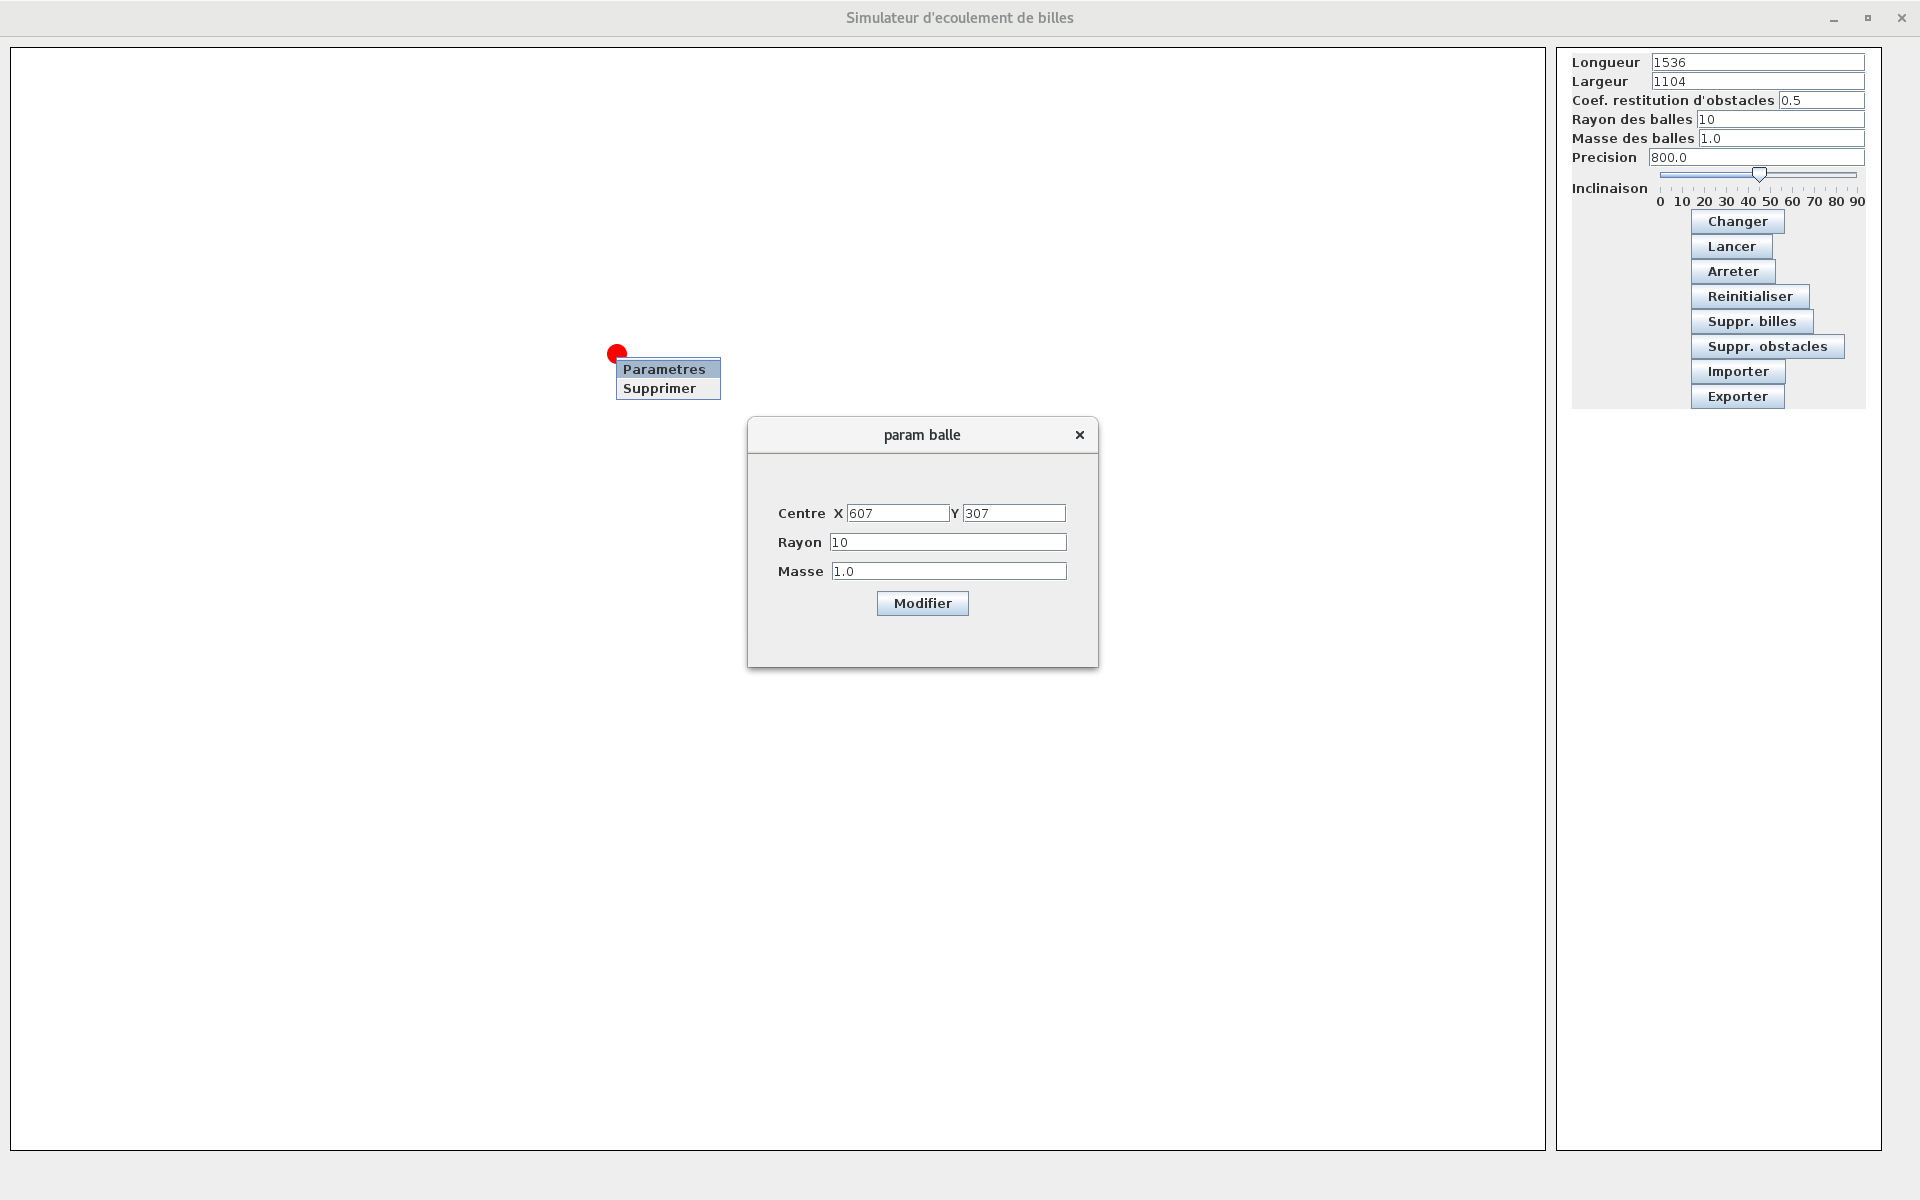
\includegraphics[scale=0.25]{modifier_bille.png}
\caption{Fenêtre de modification pour une bille}
\end{figure}

\begin{figure}[H]
\centering
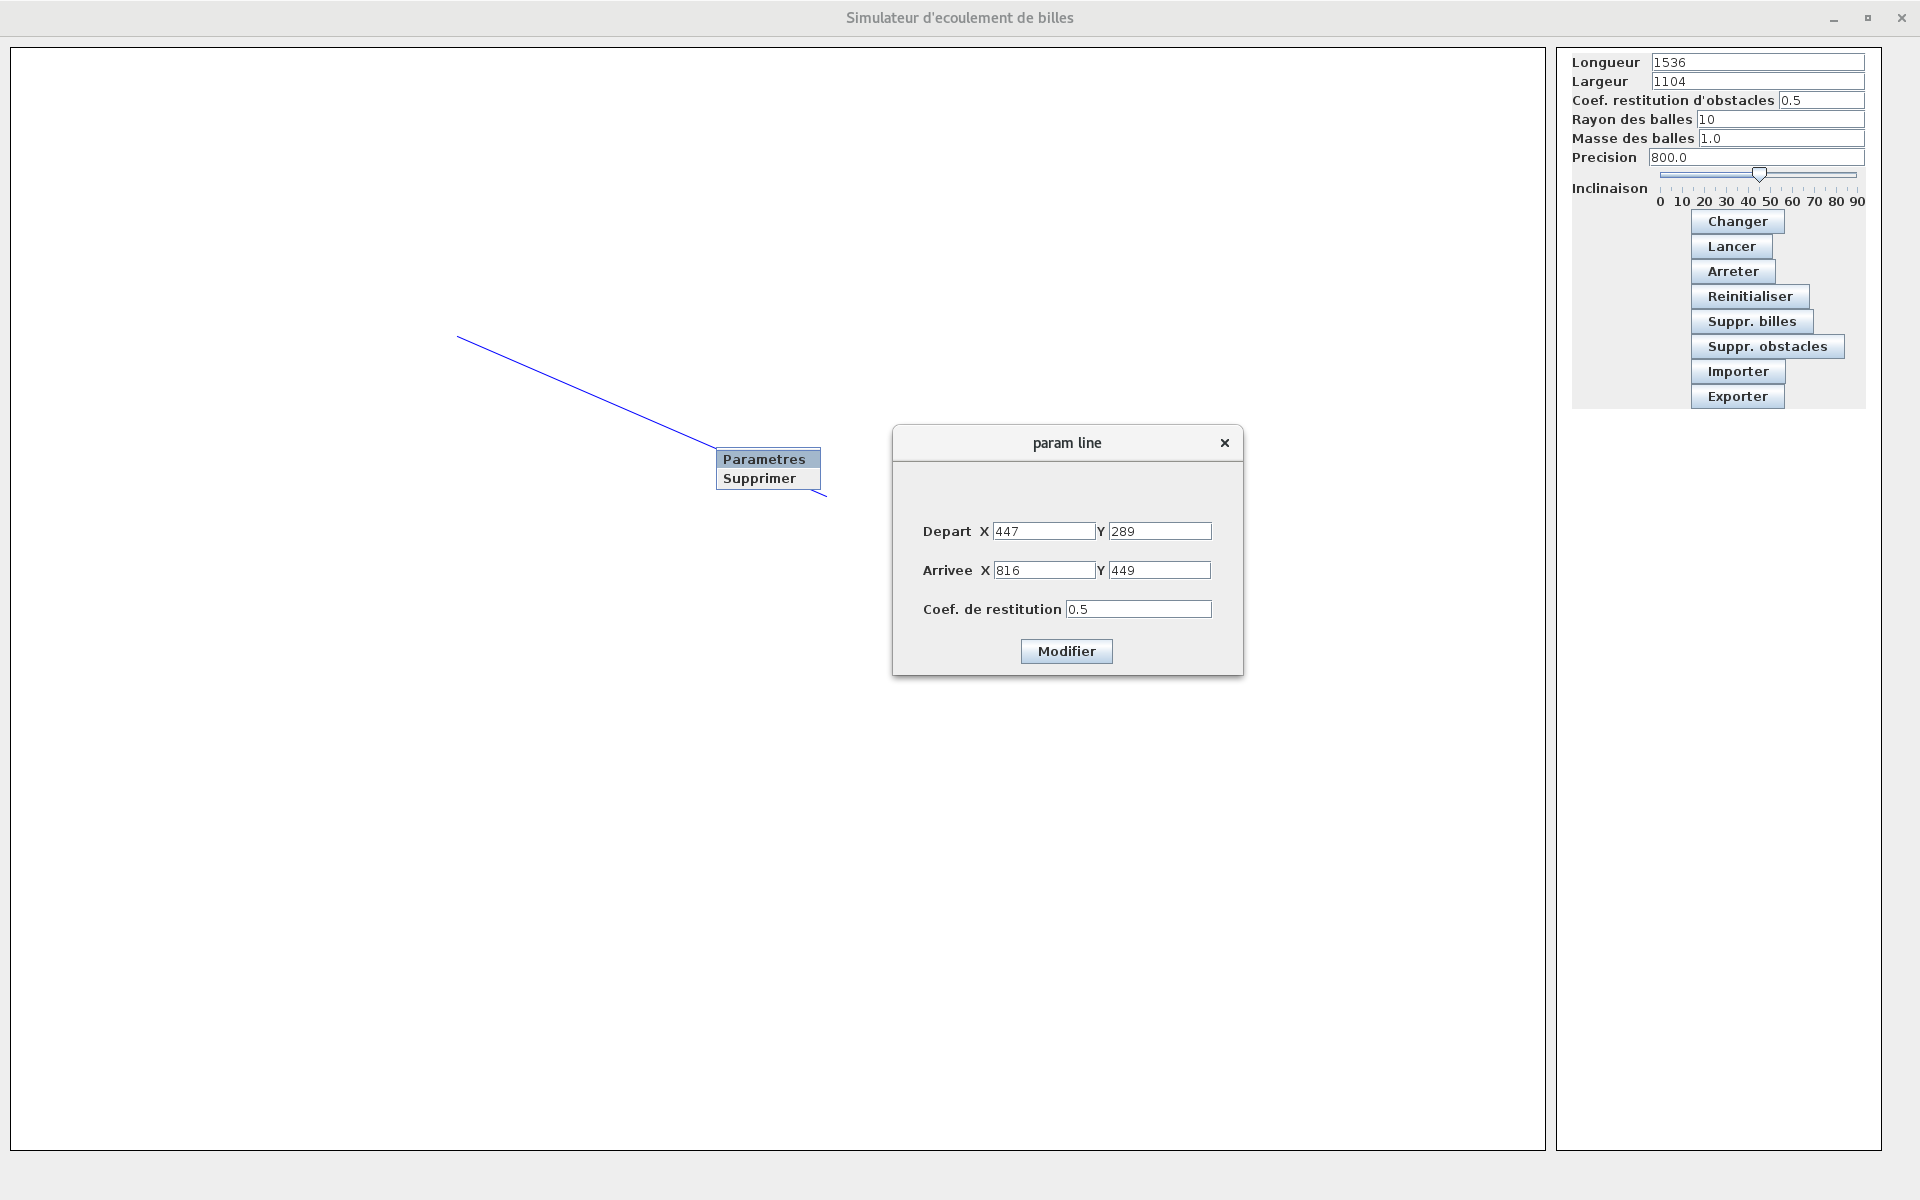
\includegraphics[scale=0.25]{modifier_obstacle.png}
\caption{Fenêtre de modification pour un obstacle}
\end{figure}

\subsubsection{Panneau de paramétrage}

Sur le panneau de paramétrage, l’utilisateur peut interagir plus globalement avec le circuit. \\

Voici les actions possibles :
\begin{itemize}
\item Champs de texte et bouton “Changer” : l’utilisateur peut modifier, à l’aide de champs de texte, les caractéristiques affichées à l’écran (longueur et largeur du circuit, coefficient de restitution des obstacles, rayon et masse des billes, précision du moteur physique). Une fois que l’utilisateur a rempli les champs comme il le souhaite, il clique sur le bouton “Changer” afin d’appliquer ces changements. Tous les changements s’appliquent pour les prochains objets créés, donc les objets actuellement sur le circuit au moment du changement ne sont pas affectés par ces modifications. En ce qui concerne le champ “Precision”, ce nombre représente l’échelle du pas de temps utilisé pour le moteur physique : plus la précision est grande, plus la simulation sera fine mais lente ; à l’inverse, plus la précision est petite, plus la simulation sera rapide mais grossière.
\item Slider "Inclinaison” : l’utilisateur peut changer en temps réel l’inclinaison du circuit. 90 correspond à un circuit vertical (les billes tombent en chute libre) et 0 à un circuit plat. L’inclinaison est modifiable au cours d’une simulation.
\item Boutons “Lancer” et “Arreter” : ces deux boutons permettent respectivement à l’utilisateur de lancer et arrêter la simulation. Lorsque la simulation est en cours d’exécution, le bouton “Lancer” est de couleur verte, et il est impossible de cliquer sur d’autres boutons du panneau de paramétrage (sauf “Arreter” et le slider “Inclinaison”) ou de cliquer sur le panneau de dessin. Lorsque la simulation n’est pas en cours d’exécution, le bouton “Arreter” est de couleur rouge (ou sans couleur si aucune simulation n’a été lancée depuis le lancement de l’application) et il est à nouveau possible de cliquer sur les boutons du panneau de paramétrage ou sur le panneau de dessin.
\item Boutons “Reinitialiser”, “Supp. billes” et “Supp. obstacles” : l’utilisateur peut supprimer un ensemble d’objets du circuit en utilisant ces boutons. Le bouton “Reinitialiser” supprime tous les objets (billes et obstacles), alors que les deux autres ne suppriment que leur propre catégorie d’objets. Le bouton “Reinitialiser” ne fait rien de plus que de supprimer les objets, il ne va, par exemple, pas remettre les dimensions du circuit ou l’inclinaison par défaut.
\item Boutons “Importer” et “Exporter” : l’utilisateur peut exporter et importer des circuits. Les détails de l’import et de l’export sont expliqués dans la sous-partie “Gestion de fichiers”.
\end{itemize}

\subsection{Simulation}

Lorsque l’utilisateur lance la simulation, les billes du circuit dans le panneau de dessin commencent à bouger. Les billes laissent derrière elles une trace verte représentant leur parcours au cours de la simulation.

\begin{figure}[H]
\centering
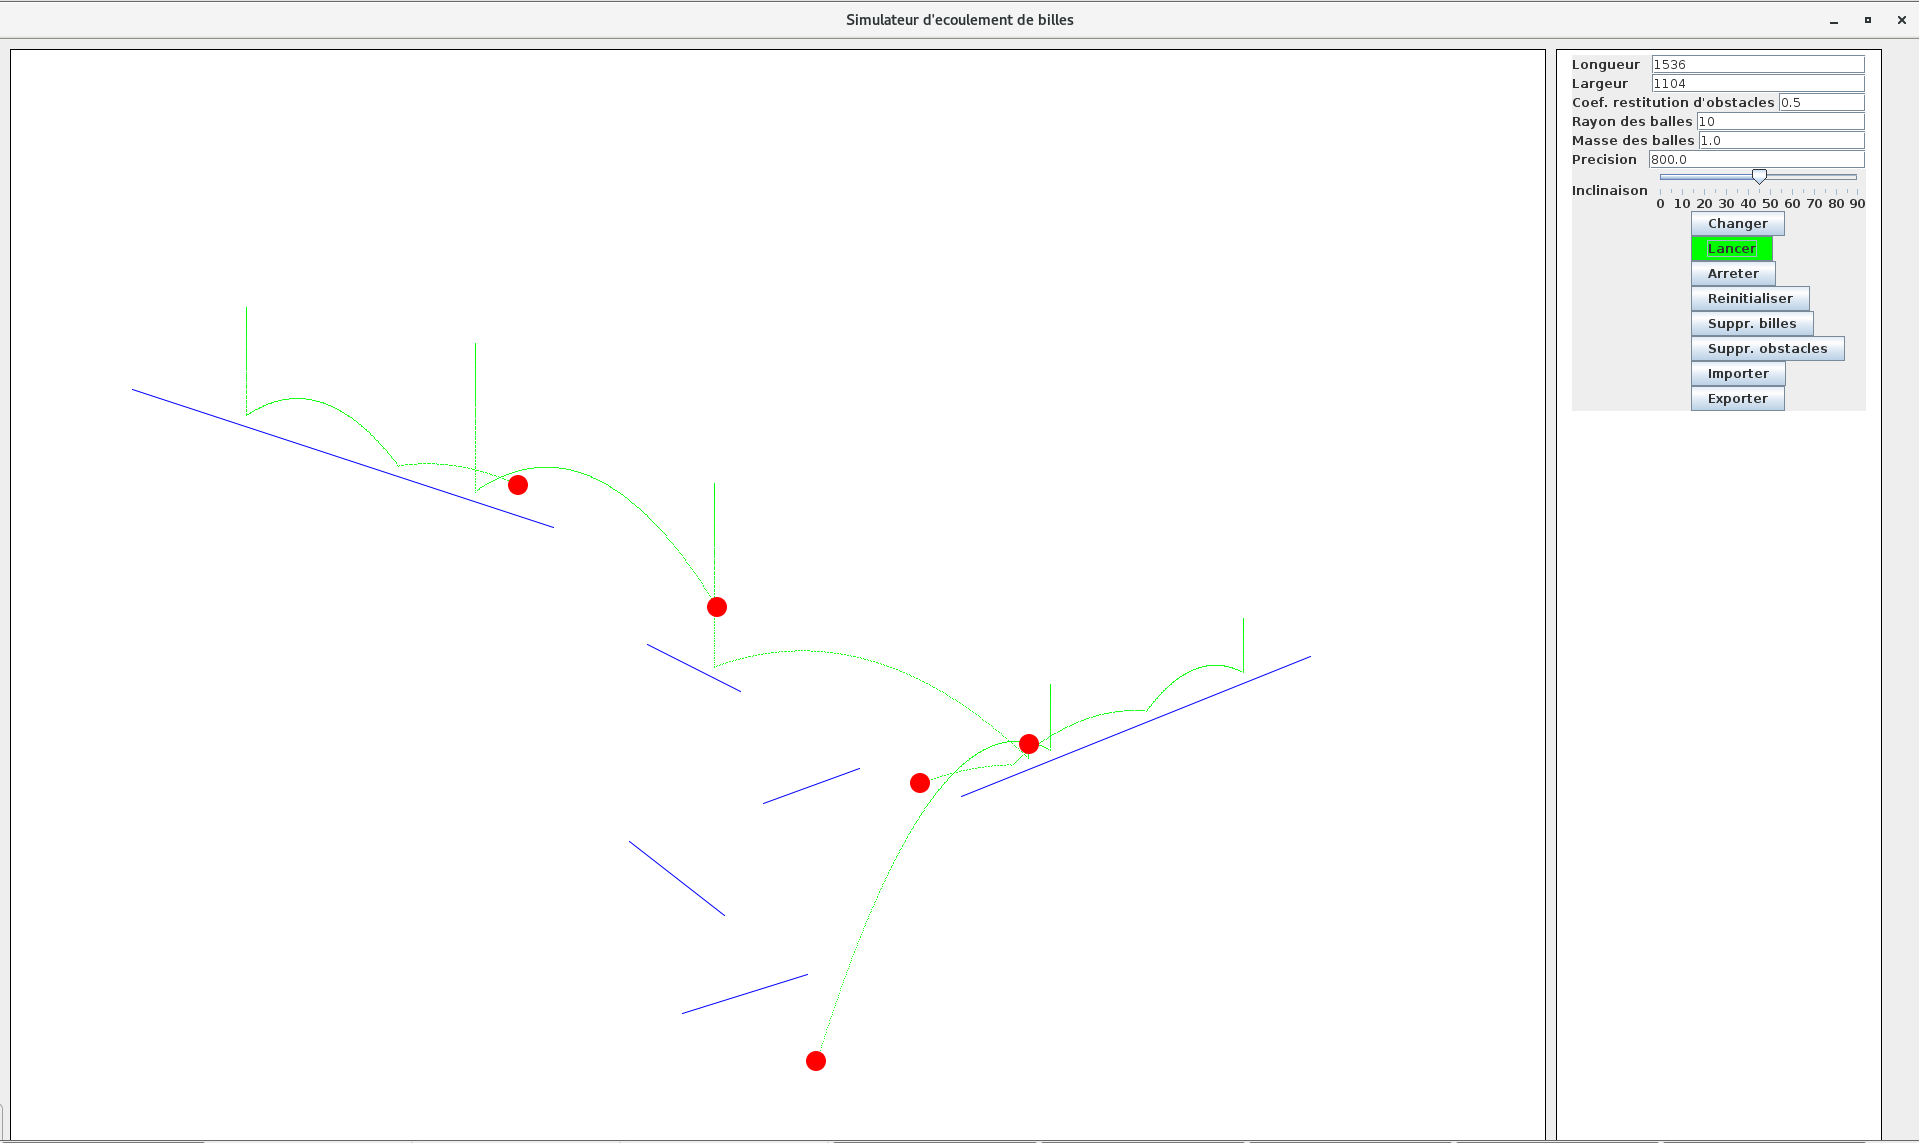
\includegraphics[scale=0.25]{simulation.png}
\caption{Exemple de simulation en cours d'exécution}
\end{figure}

Au cours de cette simulation, les billes vont interagir et potentiellement entrer en collision avec d’autres billes ou des obstacles. Le moteur physique calcule la résolution de ces collisions afin d’obtenir un comportement de billes se rapprochant de la réalité.

\newpage
\subsection{Gestion de fichiers}

\subsubsection{Export}

Le circuit est exporté dans un fichier au format XML qui aura sa propre extension “.pdp”, permettant de reconnaître un fichier associé à l’application. L’export sauvegarde toutes les données du circuit : dimensions, inclinaison, précision, ainsi que l’ensemble des objets avec chacun l’ensemble de leurs caractéristiques individuelles, traces comprises.

\begin{figure}[H]
\centering
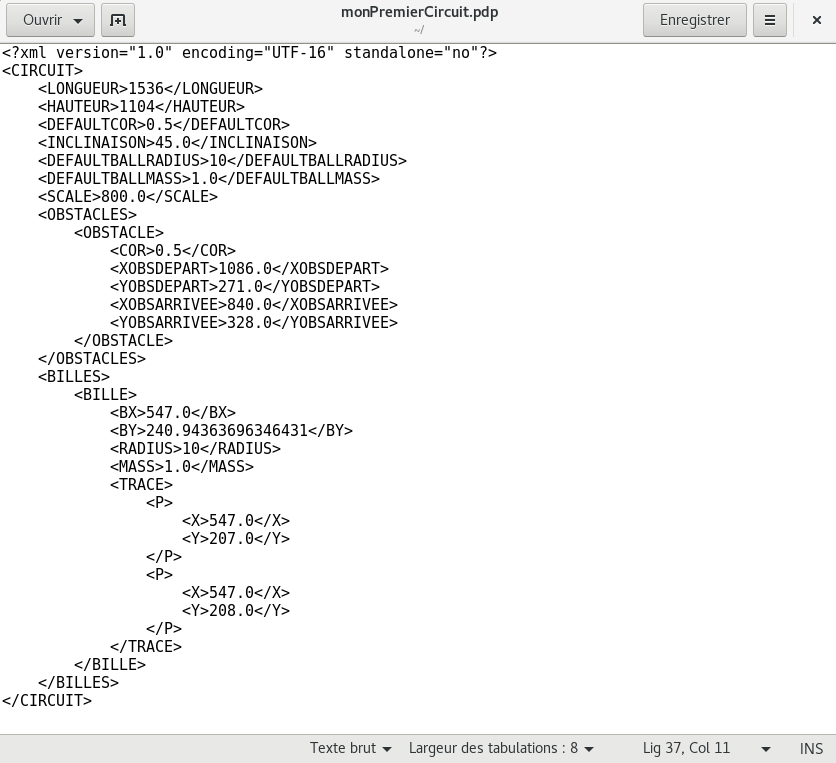
\includegraphics[scale=0.5]{fichier_pdp.png}
\caption{Exemple de fichier d'export de circuit}
\end{figure}

\subsubsection{Import}

Lors de l’import, l’application lit le fichier d’export, ce qui lui permet de recréer le circuit importé de façon identique. Cependant, comme la fonction d’import est censée permettre de considérer un circuit exporté comme un nouveau circuit initial, les traces ne sont pas importées. De plus, si le circuit importé est trop grand par rapport à l’écran de l’utilisateur, alors le circuit est rogné sur le côté droit et sur le bas (mais le fichier utilisé pour l’import n’est pas modifié).

\section{Analyse du fonctionnement}

\subsection{Fonctionnement}

\subsubsection{Déplacement des billes}

\paragraph{Gravité}

Au lancement de l’exécution, les billes sont déplacées vers le bas du circuit à cause de l’accélération de la gravité. Cette accélération dépend de l’inclinaison du circuit qui varie entre 0 et 90 degrés. Lorsque l’inclinaison vaut 0 degré, l’accélération est nulle et les billes ne bougent pas. A l’inverse, lorsque l’inclinaison vaut 90 degrés, la bille est en chute libre et son accélération est égale à la gravité.

\paragraph{Événements externes}

Lors de leur écoulement, les billes peuvent entrer en collision avec des obstacles, ce qui va modifier leur trajectoire. Elles peuvent également entrer en collision avec d’autres billes. La détection et la résolution des collisions sont détaillées dans la partie suivante.

\paragraph{Sortie d'écran}

Lorsqu’une bille sort de l’écran on considère qu’elle n’est plus sur le circuit. On arrête de la déplacer.

\subsubsection{Collisions}

\paragraph{Gestion}

\subparagraph{Détection}

À chaque pas de temps, après avoir déplacé une bille, on vérifie si elle entre en collision avec un obstacle ou une bille. Si c’est le cas, il faut traiter cette collision.

\subparagraph{Résolution}

La résolution d’une collision bille-obstacle est différente de celle bille-bille. \\

Dans le premier cas, on commence par replacer la bille sur l’obstacle si elle le chevauche. Ensuite, on calcule l’angle de rebond à partir de l’angle d’arrivée de la bille et l’angle de la normale avec l’obstacle. La nouvelle vitesse est calculée en fonction du coefficient de restitution de l’obstacle qui atténue uniquement la composante Y du vecteur vitesse. Dans le cas où ce coefficient vaut 1, la vitesse finale est la même que la vitesse initiale. En connaissance de l’angle de rebond et de la vitesse finale,  on met à jour le vecteur vitesse et la bille sera déplacée correctement au prochain pas de temps. \\

Dans le cas d’une collision bille-bille. On récupère la direction des deux billes, puis on calcule l’angle de collision. On calcule ensuite les nouvelles directions en fonction de leur direction initiale et l’angle de collision. Les vitesses finales dépendent de la masse des billes. On replace les billes si elles se chevauchent, selon la distance minimum entre les deux centres et  leur masse. Enfin, on met à jour les vecteurs vitesses.

\paragraph{Optimisation}

Nous avons décidé d’utiliser un Quadtree pour partitionner l’espace 2D de notre circuit car cette solution répond parfaitement à nos besoins. Son implémentation a été réalisée en suivant le tutoriel présent à la référence \cite{07}. A chaque appel de la fonction \texttt{run()} qui va déplacer toutes les billes d’un pas de temps, on vide le Quadtree puis on rajoute toutes les billes dedans. Ensuite, plutôt que de tester la collision de chaque bille avec toutes les autres, on teste la collision uniquement avec celles voisines (situées dans la même région), renvoyées par le Quadtree.

\newpage
\subsubsection{Traces}

\paragraph{Implémentation}

Lorsqu’une bille se déplace lors d’une simulation, elle laisse derrière elle sa trace, ce qui permet de connaître le parcours qu’elle a effectué au cours de cette simulation.
La trace d’une bille est implémentée par une liste de points, chacune correspondant à la position du centre de la bille à un instant de la simulation. Un point est ajouté à la liste à chaque fois que la bille se déplace lors d’un pas de temps. Cela signifie que lorsqu’une bille n’a pas bougé (ou quasiment pas bougé) lors d’un pas de temps, le point représentant son centre à cet instant-là n’est pas ajouté à la liste, puisqu’un point de mêmes coordonnées est déjà censé y être.

\paragraph{Affichage}

Lors de la mise à jour de l’affichage, la méthode par défaut est de tout effacer puis tout réafficher. Cependant, au cours de l’exécution de la simulation, le nombre de points représentant la trace d’une bille ne cesse d’augmenter. Cela voudrait dire qu’en utilisant cette méthode de mise à jour, il faudrait parcourir toutes les listes de points formant la trace de chaque bille (qui deviennent donc de plus en plus grandes) afin de toutes les réafficher, et ce à chaque pas de temps. Il devient donc très difficile d’avoir une simulation fluide en mettant à jour l’affichage de cette façon. \\

Nous avons donc opté pour une autre méthode : le passage par une image bufferisée. Dans cette image sont stockés les objets n’étant pas amenés à être changés de place : les obstacles et les traces (chaque fois qu’une bille se déplace, on ajoute sa nouvelle trace à l’image bufferisée, on n’efface rien de cette dernière). \\

Le but de cette méthode est que lorsque la mise à jour de l’affichage est effectuée, on efface tout, on affiche l’image bufferisée, puis on affiche les billes par-dessus. La différence avec la première méthode est que, là où on devait réafficher toutes les traces à chaque pas de temps avant, on ajoute désormais uniquement le dernier point de chaque trace à chaque pas de temps à l’image bufferisée. \\

Cependant, bien que cette méthode améliore nettement les performances de l’application, elle reste toutefois coûteuse par rapport au reste des opérations d’une simulation.

\newpage
\subsection{Limites}

\subsubsection{Collisions du moteur physique}

\paragraph{Bugs}

Une bille traverse un obstacle. Cela arrive lorsqu’une bille possède une grande vitesse. Si la distance parcourue lors d’un pas de temps est supérieure à deux fois le rayon de la bille, il peut arriver que la collision ne soit pas détectée. De même, si cette distance est supérieure au rayon et inférieure à deux fois le rayon, il peut arriver que le centre de la bille se trouve de l’autre côté de l’obstacle lorsque la collision est détectée. Dans ce cas la bille est replacée en dessous de l’obstacle au lieu d’être replacée dessus.

\begin{figure}[H]
\centering
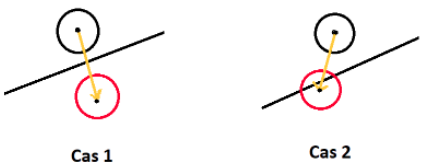
\includegraphics[scale=1]{bug_1.PNG}
\caption{Schémas du bug d'une bille passant à travers un obstacle}
\end{figure}

%===========================
\begin{figure}[H]
\centering
\begin{tikzpicture}
    \begin{axis}[
        xlabel=$temps\ .ms$,
        ylabel=$vitesse\ .pixel$]
    \addplot[smooth,mark=*,blue] 
    	plot coordinates {      
        	(0,0)
        	(15,0.008)
        	(1500,0.866)
            (3000,1.734)
    };
    \addlegendentry{800}
    \addplot[smooth,color=red,mark=x]
        plot coordinates {
        	(0,0)
        	(15,0.017)
        	(1500,1.734)
            (3000,3.467)
        };
    \addlegendentry{400}
    \addplot[smooth,color=green,mark=+]
        plot coordinates {
        	(0,0)
        	(15,0.035)
        	(1500,3.467)
            (3000,6.934)
        };
    \addlegendentry{200}
    \end{axis}
\end{tikzpicture}
\caption{Evolution de la vitesse des billes en fonction de l'échelle et du temps}
\end{figure}
%===========================

Ce bug est le seul que nous ayons réussi à mettre en évidence, néanmoins, il est possible que d'autres subsistent.

\newpage


\paragraph{Mécanique du moteur}

Notre moteur physique est basé sur la simulation discrète synchrone qui est reliée à un pas de temps. C’est-à-dire qu’à chaque pas de temps, on déplace les billes puis on exécute les vérifications de collisions après. Comme il est expliqué dans \cite{01}, ce type de moteur physique est répandu car il est “simple” à programmer et donne des résultats suffisants dans la plupart des utilisations. Cependant, il possède des limites en terme de précision car on accumule des approximations. Il faut souvent replacer les objets ou revenir en arrière et réduire le pas de temps. \\

Un autre point qui n’est pas pris en compte est la gestion des événements dans le temps. Par exemple, si deux billes sont au repos et en contact, et qu’une bille vient entrer en collision dans les deux en même temps, laquelle doit-on déplacer en premier ? Dans notre cas, on ne gère la collision qu’avec une seule bille. Pour gérer une collision entre plusieurs billes, il aurait fallu implémenter un moteur physique basé sur la simulation discrète asynchrone dans laquelle les événements (ici collisions) sont déterminés avant le déplacement.

\subsubsection{Interface graphique}

\paragraph{Ergonomie}

\subparagraph{Responsivity}

“Responsivity” correspond à l’adaptation de l’affichage de l’application, en fonction de la taille de la fenêtre d’affichage. Par exemple, diminuer la taille de la fenêtre pourrait redimensionner les panneaux de dessin et de paramétrage afin que tout reste visible à l’écran.
En l'occurrence, notre application n’est pas responsive : l’application est adaptée pour être affichée à la taille de l’écran de l’utilisateur, uniquement en plein écran. Il est déconseillé de diminuer la taille de la fenêtre, sous risque de ne plus voir une partie de l’application.

\subparagraph{Lisibilité}

Dès que le nombre de billes dans notre simulation est important, il devient difficile de distinguer à quelle bille correspond quelle trace. En effet, actuellement, toutes les billes de l’application sont rouges et toutes les traces de billes sont vertes.

\paragraph{Taille du circuit}

Dans l’application, la taille du panneau de dessin correspond exactement à la taille du circuit. Cela signifie qu’il est impossible de créer un circuit plus grand qu’un certain pourcentage de la taille de l’écran de l’utilisateur.
De plus, si un circuit trop grand par rapport à l’écran de l’utilisateur est importé, la partie qui dépasse sera rognée sur la droite et sur le bas du circuit.

\paragraph{Bibliothèque d'affichage}

Notre application utilise la bibliothèque d’affichage SWING. Cette bibliothèque n’est pas adaptée à un rafraîchissement rapide et régulier. En outre, elle n’est pas faite pour de l’affichage en temps réel. C’est sans doute la raison pour laquelle les lenteurs de notre application sont liées aux fonctions d’affichage (cela sera vu plus en détails dans la partie Tests de ce document).

%%% PARTIE 5 : ARCHITECTURE DU LOGICIEL %%%
\chapter{Architecture du logiciel}

\section{Description}

Dans cette partie, nous présentons les choix d'architecture réalisés pour le développement de l'application.

\subsection{Structure Modèle-Vue-Contrôleur (MVC)}

Notre application utilisant une interface graphique, il nous est paru naturel d'utiliser une structure applicative Modèle-Vue-Contrôleur (MVC). Cette structure permet de séparer les fonctionnalités de notre application dans des classes en fonction de l'intention de ces fonctionnalités. 
\begin{itemize}
\item Modèle : contient les données à afficher
\item Vue : implémente l'interface permettant d'afficher les données
\item Contrôleur : définit les opérations effectuées par l'utilisateur et les traitements à effectuer sur les données
\end{itemize}

Ainsi, dans notre application, notre circuit et les objets qui le composent forment notre modèle. Les actions que peut effectuer l'utilisateur, les traitements qui y sont liés et la gestion de la simulation forment notre contrôleur. Enfin, tous les objets liés à l'affichage et à la paramétrabilité de l'application forment notre vue.

\subsection{Organisation des classes}

\begin{figure}[H]
\centering
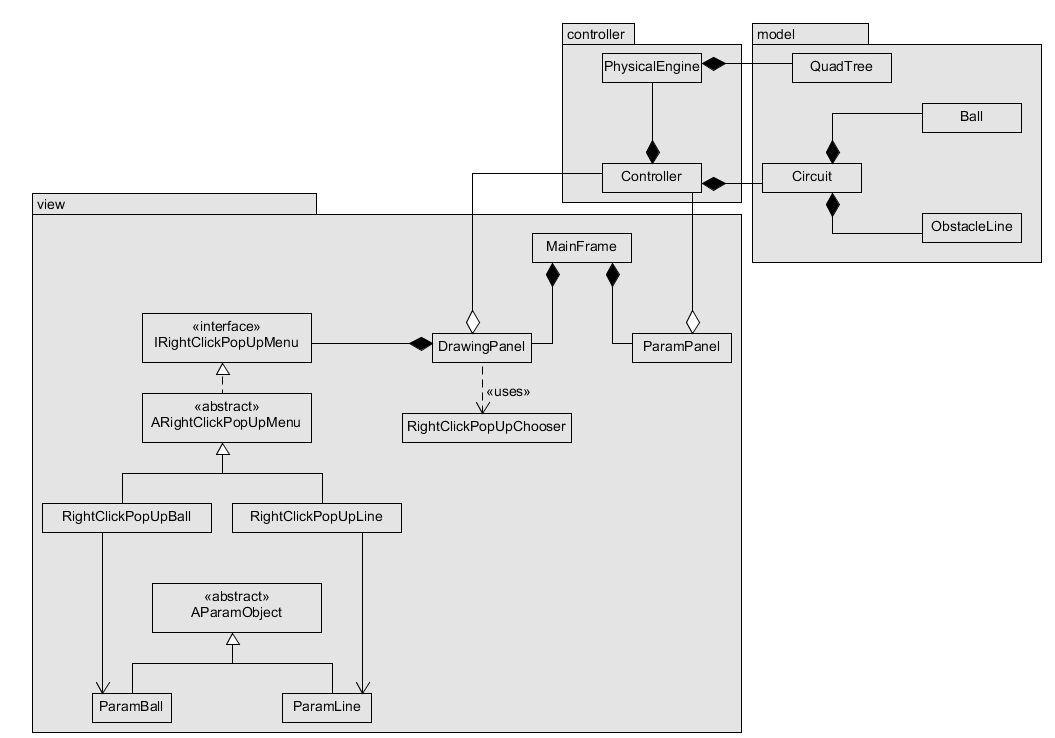
\includegraphics[scale=0.65]{uml.png}
\caption{Diagramme de classes de l'application}
\end{figure}

Ce diagramme de classes contient toutes les classes de notre application exceptées les classes "AnimationTimer" et "Vector" du modèle car elles ne répondent pas directement à un besoin. Il n'y a donc pas de raison de les commenter ici.

Pour plus d'information sur ces classes, voir la partie "Présentation des classes" de ce document.

\subsubsection{Modèle}

Les classes Ball et ObstacleLine sont des composantes de la classe Circuit. Notre circuit implémentant le plateau sur lequel nos objets vont évoluer, il a besoin de posséder la liste des objets de notre simulation.

\subsubsection{Vue}

La classe principale de l'application est la classe MainFrame. C'est lorsqu'on crée une instance de cet objet qu'une fenêtre s'ouvre et l'application démarre. \\

Une MainFrame est composée d'un DrawingPanel (panneau de dessin qui va afficher le circuit) et d'un ParamPanel (panneau permettant de paramétrer le circuit et d'effectuer certaines actions comme lancer l'exécution ou importer un circuit). \\

DrawingPanel et ParamPanel étant des objets permettant d'afficher ou de paramétrer un circuit, ils ont besoin d'avoir accès à certaines informations du modèle. Pour cela, ils récupèrent une référence sur l'instance du Controller à travers lequel ils pourront obtenir les informations ou effectuer les actions dont ils ont besoin. \\

La classe RightClickPopUpChooser est un pseudo-Visitor. Dans le DrawingPanel, on veut que lorsqu'on clique droit sur un objet du circuit, on ouvre un pop up correspondant au type d'objet sur lequel on a cliqué. Le rôle de la classe RightClickPopUpChooser est de recevoir un point du circuit et, selon le type de l'objet sur lequel il est (s'il est sur un objet), créer et renvoyer une instance de  IRightClickPopUpMenu correspondant au type d'objet reçu. Le DrawingPanel récupère ensuite cette instance dans son attribut correspondant et affiche le pop up. \\

Enfin, étant donné que chaque IRightClickPopUpMenu de notre application doit être capable de demander la suppression de l'objet sur lequel il est invoqué ou d'ouvrir une fenêtre de paramétrage de cet objet, il y a une association entre les RightClickPopUpX et les ParamX (X étant "Ball" ou "Line").

\subsubsection{Contrôleur}

La classe "Controller" est un Singleton. Ce design pattern garantit que cette classe n'a qu'une seule instance et fournit un point d'accès global à celle-ci. C'est l'instance de notre Controller qui crée et possède le Circuit du modèle. C'est aussi elle qui va définir les services que l'on propose à l'utilisateur (la vue) pour interagir avec ce circuit. Enfin, si l'utilisateur le demande, c'est lui qui va lancer l'exécution de la simulation d'écoulement de billes à travers le "PhysicalEngine".

Le PhysicalEngine permet d'exécuter la simulation d'écoulement des billes.

\subsection{Améliorations}

Ici, nous présentons les améliorations d'architecture majeures auxquelles nous avons pensé.

\subsubsection{Interface Movable}

Notre application ne possède qu'un seul type d'objet capable de se déplacer : Ball. Pour cette raison, nous n'avons pas créé d'interface "Movable" permettant de définir un comportement qui serait commun à tous les objets capables de se déplacer dans notre application. 

Dans un souci d'extensibilité, il faudrait donc rajouter une interface IMovable, contenant au minimum les méthodes \texttt{step(Vector):void} permettant à un objet de se déplacer et \texttt{contains(Point):bool} permettant de savoir si un Point est dans l'objet en question.

On pourrait alors définir une liste d'objets "IMovable" plutôt que "Ball" dans le Circuit.

\subsubsection{Interface Obstacle}

Notre application ne possédant qu'un seul type d'obstacle (ObstacleLine), nous n'avons pas créé d'interface "Obstacle" définissant le comportement minimal d'un obstacle. 

Là aussi, dans un soucis d'extensibilité, nous pourrions rajouter cette interface et ainsi définir les services que doit rendre chaque nouvelle forme d'obstacle dans notre application. Cette interface devrait au minimum contenir la méthode \texttt{contains(Point):bool} qui sera utilisée pour détecter les collisions.

On pourrait alors définir une liste d'objets "IObstacles" plutôt que "ObstacleLine" dans le Circuit.

\subsubsection{Implémentation d'Observer-Observable}

Observer est un design pattern dont le but est de définir une interdépendance (de type un à plusieurs) de telle sorte que, lorsqu'un objet change d'état, tous ceux qui en dépendent sont notifiés et automatiquement mis à jour.

Nous nous sommes rendus compte que parfois, la communication entre notre modèle, notre vue et notre contrôleur n'était pas toujours optimale. Par exemple, certaines classes devaient parfois posséder une référence sur un objet alors qu'elles ne l'utilisaient jamais. Elles conservaient cette référence afin de la passer à un autre objet qu'elles auraient créé et qui, lui, en aurait besoin.

En implémentant le design pattern Observer, nous pourrions améliorer la communication entre nos objets. Notre modèle serait, à ce moment-là, observé par notre vue. Ainsi, chaque fois que le modèle serait modifié et, en fonction de la modification apportée, chaque objet de notre vue qui l'observait pourrait effectuer le traitement correspondant afin d'actualiser l'affichage pour l'utilisateur. Ainsi, chaque objet de la vue observerait ce dont il a besoin dans le modèle et les communications seraient simplifiées.

\subsubsection{Opérations Vue-Contrôleur}

Certaines des opérations ont été maladroitement implémentées. Par exemple, pour ajouter un objet dans le circuit, la vue réalise tous les tests nécessaires en appelant les méthodes du contrôleur. Puis, si ces tests réussissent, elle appelle la méthode \texttt{add():void} du contrôleur sur l'objet en création ; la méthode \texttt{add():void} du contrôleur ne faisant rien de plus qu'appeler celle du circuit.

Ce comportement est maladroit car il aurait été plus logique que la vue appelle directement la méthode \texttt{add():void} du contrôleur et que ce soit celui-ci qui réalise les tests à effectuer lors d'un ajout d'objet dans le circuit.

\section{Présentation des classes}

Dans cette partie, nous présentons chaque classe (objectifs, attributs et méthodes) de l'application à la manière d'une documentation fonctionnelle.

\subsection{Package model}

\subsubsection{Classe Vector}

Notre moteur physique met en œuvre des forces. En physique, une force est représentée par un vecteur. Pour cette raison, nous avons besoin d'implémenter une classe permettant de représenter un vecteur et capable de réaliser certaines opérations sur celui-ci.

\paragraph*{Attributs}
\begin{itemize}
\item \texttt{double \_x} : taille du vecteur selon l'axe X
\item \texttt{double \_y} : taille du vecteur selon l'axe Y
\end{itemize}

\paragraph*{Méthodes}
\begin{itemize}
\item \texttt{Vector vectorSum(Vector A, Vector B)} : retourne un vecteur dont les valeurs est la somme des vecteurs A et B.
\item \texttt{Vector vectorSubstract(Vector A, Vector B)} : retourne un vecteur dont les valeurs est la différence des vecteurs A et B.
\item \texttt{double dotProduct(Vector A, Vector B)} : retourne le produit scalaire des vecteurs A et B.
\item \texttt{Vector vectorProductConstant(Vector A, double val)} : retourne un vecteur dont les valeurs  \_x et \_y ont été multipliées par "val".
\item \texttt{Vector Product(Vector A, Vector B)} : retourne le produit des vecteurs A et B.
\end{itemize}

\subsubsection{Classe ObstacleLine}

Cette classe implémente les obstacles dont la forme est un segment.

\paragraph*{Attributs}
\begin{itemize}
\item \texttt{double \_COR} : coefficient de restitution de l'obstacle 
\item \texttt{Point \_begin} : point de départ du segment
\item \texttt{Point \_end} : point d'arrivée du segment
\end{itemize}

\paragraph*{Méthodes}
\begin{itemize}
\item \texttt{Boolean contains(Point p)} : cette méthode permet de déterminer si le point "p" passé en paramètre est sur l'ObstacleLine. Pour savoir cela, on utilise l'inégalité triangulaire : si la distance(\_begin, p)  + distance(p, \_end) = distance(\_begin, \_end), alors p est entre \_begin et \_end et p appartient à l'obstacle.
\item \texttt{Boolean isNearPoint(Point p)} : cette méthode permet de déterminer si le point "p" est proche de l'obstacle. Cette méthode est préférée à \texttt{contains} lorsque l'on veut savoir si un clic droit a été effectué sur un ObstacleLine. Ce dernier étant fin de 1 pixel, il est difficile de cliquer exactement dessus.
\end{itemize}

\subsubsection{Classe Ball}

Objet principal de notre application, la classe Ball implémente la numérisation des billes dont nous devons simuler l'écoulement.

\paragraph*{Attributs}
\begin{itemize}
\item \texttt{Vector \_location} : ce vecteur représente la position du centre de la bille dans le circuit. 
\item \texttt{Vector \_velocity} : ce vecteur représente la vitesse de la bille (une vitesse verticale et une vitesse horizontale).
\item \texttt{double \_mass} : masse de la bille
\item \texttt{int \_radius} : rayon de la bille
\item \texttt{ArrayList<Point> \_track} : liste de points représentant le tracé de la bille au cours de la simulation. Chaque fois que la bille va se déplacer, on va sauvegarder sa nouvelle position dans cette liste.
\end{itemize}

\paragraph*{Méthodes}
\begin{itemize}
\item \texttt{Boolean contains(Point p)} : détermine si le point "p" passé en paramètre est dans la bille. Pour cela, on regarde simplement si la distance entre le centre de la bille et "p" est supérieure ou inférieure au rayon de la bille.
\item \texttt{void step()} : calcule la nouvelle position et la nouvelle vitesse de la bille en fonction de l'accélération de la gravité, de ses coordonnées et de sa vitesse au pas de temps précédent. Si l'ancienne et la nouvelle position transtypées en entier sont différentes, on sauvegarde la nouvelle position dans "\_track". On transtype en entier les coordonnées avant de les tester afin d'arrondir leur valeur et ainsi diminuer le nombre de points à insérer dans la liste. Évidemment, nous diminuons la précision de nos traces en effectuant cette opération mais c'est un mal nécessaire afin de permettre un export de ces données. Lors d'un export, chaque point de la trace de chaque bille est inscrit dans le fichier et, en gardant la précision des doubles, les fichiers devenaient trop vite démesurément lourds.
\end{itemize}

\newpage
\subsubsection{Classe Circuit}

Cette classe représente le terrain sur lequel vont être posés et vont évoluer nos objets. C'est aussi la classe que nous allons vouloir exporter ou importer.

\paragraph*{Attributs}
\begin{itemize}
\item \texttt{int \_width} : longueur du circuit.
\item \texttt{int \_height} : hauteur du circuit.
\item \texttt{ArrayList<Ball> \_balls} : liste des billes du circuit.
\item \texttt{ArrayList<ObstacleLine> \_lines} : liste des obstacles du circuit.
\item \texttt{double \_gravitation} : valeur de la force de gravité (avec une précision de 1E-5).
\item \texttt{Vector \_gravityAcceleration} : vecteur représentant la force de gravité dans notre simulation. C'est donc la force de gravité atténuée par l'inclinaison du circuit.
\item \texttt{double \_scale} : échelle de notre simulation. Nous divisons nos vitesses et accélérations par cette valeur. En outre, plus cette valeur est grande, plus les pas de déplacement de la simulation sont petits, ce qui permet d'éviter certaines incohérences telles que le passage de billes dont la vitesse est élevée à travers un obstacle.
\item \texttt{double \_defaultInclination} : inclinaison du circuit
\item \texttt{double \_defaultCOR} : coefficient de restitution par défaut des obstacles
\item \texttt{double \_defaultBallRadius} : rayon par défaut des billes
\item \texttt{int \_defaultBallMass} : masse par défaut des billes
\end{itemize}

\paragraph*{Méthodes}
\begin{itemize}
\item \texttt{void toExport(File f)} : sauvegarde les données du circuit et de chaque bille et obstacle qui le compose dans le fichier passé en paramètre. Les données sont sauvegardées au format XML. Les fonctions \texttt{void saveCircuitXML}, \texttt{void saveBallsXML} et \texttt{void saveObstaclesXML} font parties de la fonction \texttt{toExport}. Leur séparation est uniquement due à un soucis de lisibilité.
\item \texttt{void toImport(File f)} : charge les données d'un circuit à partir du fichier passé en paramètre. On lit le fichier au format XML sans vérifier la validité de l'arborescence du fichier car on part du principe que si le fichier est importé, c'est qu'il a l'extension ".pdp" donc il a été généré par notre application et possède déjà la bonne arborescence. Les fonctions \texttt{void importCircuitXML}, \texttt{void importBallsXML} et \texttt{void importObstaclesXML} font partie de la fonction \texttt{toImport}. Leur séparation est uniquement due à un souci de lisibilité.
\end{itemize}

\subsubsection{Classe QuadTree}

Cette classe permet l'optimisation de la détection des collisions en réduisant le nombre de calculs à réaliser via un partitionnement de l'espace.

\paragraph*{Attributs}
\begin{itemize}
\item \texttt{int \_MAX\_OBJECTS} : nombre maximum d'objets dans une région. Lorsque cette limite est atteinte, si un nouvel objet est ajouté, la région se divise en 4 sous-régions.
\item \texttt{int \_MAX\_LEVELS} : profondeur maximale du Quadtree.
\item \texttt{int \_level} : niveau de profondeur du nœud courant dans le Quadtree (nœud représenté lui-même par un objet Quadtree).
\item \texttt{List<Ball> \_objects} : liste des billes situées dans la région représentée par le Quadtree.
\item \texttt{Rectangle \_bounds} : rectangle représentant la région du Quadtree.
\item \texttt{QuadTree[] \_nodes} : 4 Quadtree fils représentant les 4 sous-régions du Quadtree.
\end{itemize}

\paragraph*{Méthodes}
\begin{itemize}
\item \texttt{int getIndex(Ball ball)} : renvoie la sous-région dans laquelle se situe la bille. Valeurs possibles : 0, 1, 2, 3 ou -1 si la bille ne rentre pas complètement dans une des sous-régions et, dans ce cas, on considère qu'elle fait partie de la région entière (donc des 4 sous-régions).
\item \texttt{void insert(Ball ball)} : insère la bille dans le Quadtree.
\item \texttt{void split()} : divise la région en 4 sous régions de taille identique.
\item \texttt{void clear()} : vide le Quadtree en supprimant tous les nœuds pour revenir au Quadtree initial dont la région représente le circuit entier.
\item \texttt{List<Ball> retrieve(List<Ball> returnObjects, Ball ball)} : pour une bille donnée en paramètre, renvoie la liste des billes avec lesquelles elle doit vérifier si elle est en collision.
\end{itemize}

\subsubsection{Classe AnimationTimer}

Cette classe étend la classe Timer de la bibliothèque SWING. Elle nous permet d'implémenter une horloge. On se sert de cette classe dans notre moteur physique afin d'effectuer nos calculs et les mouvements de nos objets à intervalles réguliers.

\paragraph*{Attribut}
\begin{itemize}
\item \texttt{int STEP} : nombre de millisecondes entre deux événements
\end{itemize}

\subsection{Package controller}

\subsubsection{Classe Controller}

Cette classe sert d'intermédiaire à la vue pour effectuer des opérations sur le modèle. Cette classe doit implémenter les fonctionnalités dont l'interface graphique aura besoin pour afficher et paramétrer le circuit.

C'est un Singleton, il possède donc son instance et garantit qu'elle est unique.

\paragraph*{Attributs}
\begin{itemize}
\item \texttt{Circuit \_circuit} : circuit de l'application. C'est celui que l'interface affiche et sur lequel on effectue la simulation.
\item \texttt{Controller \_instance} : unique instance de Controller qui existe au cours de l'exécution de l'application.
\item \texttt{Boolean \_isRunning} : booléen permettant de savoir si la simulation est en cours ou non.
\item \texttt{PhysicalEngine \_pe} : instance du moteur physique qui est utilisée pour exécuter la simulation.
\end{itemize}

\paragraph*{Méthodes}
\begin{itemize}
\item \texttt{Ball checkIfPointIsInBall(Point p)} : appelle la méthode \texttt{contains()} du circuit pour déterminer si le point donné en argument se trouve dans une bille du circuit, et la bille est retournée si c'est le cas. Elle est utilisée pour vérifier si l'utilisateur a cliqué sur une bille existante.
\item \texttt{ObstacleLine checkIfPointIsNearLine(Point p)} : appelle la méthode \texttt{isNearPoint()} pour déterminer si le point donné en argument se trouve près d'un obstacle du circuit, et l'obstacle est retourné si c'est le cas. Elle est utilisée lorsque l'utilisateur a cliqué près d'un obstacle existant.
\item \texttt{void removeLinesOutOfBounds(int xMin, int xMax, int yMin, int yMax)} : supprime les obstacles hors du circuit lors du redimensionnement, en comparant la position de leurs extrémités avec les dimensions données en argument.
\item \texttt{void removeBallsOutOfBounds(int xMin, int xMax, int yMin, int yMax)} : supprime les billes hors du circuit lors du redimensionnement, en comparant la position de leurs extrémités avec les dimensions données en argument.
\item \texttt{void runSimulation(DrawingPanel creationZone)} : passe le booléen \_isRunning à Vrai pour indiquer que la simulation est lancée, puis lance le moteur physique sur le panneau donné en argument. Elle est utilisée lorsque l'utilisateur clique sur le bouton "Lancer".
\item \texttt{void stopSimulation()} : passe le booléen \_isRunning à Faux pour indiquer que la simulation est stoppée, puis arrête le moteur physique. Elle est utilisée lorsque l'utilisateur clique sur le bouton "Arrêter".
\item \texttt{boolean checkIfBallIsOnExistingBall(Ball b)} : teste si la bille donnée en entrée est positionnée sur une bille du circuit, en appelant la méthode de détection de collisions bille-bille. Retourne Vrai si c'est le cas et Faux sinon.
\item \texttt{boolean checkIfBallIsOnExistingLine(Ball b)} : teste si la bille donnée en entrée est positionnée sur un obstacle du circuit, en appelant la méthode de détection de collisions bille-obstacle. Retourne Vrai si c'est le cas et Faux sinon.
\item \texttt{void checkIfBallIsOnExistingObject(Ball b)} : appelle les deux méthodes checkIfBallIsOnExistingBall(Ball b), et renvoie Vrai si au moins l'une des deux renvoie Vrai. Sinon, c'est Faux qui est renvoyé.
\item \texttt{boolean checkIfLineIsOnExistingBall(ObstacleLine o)} : teste si l'obstacle donné en entrée est positionné sur une bille du circuit, en appelant la méthode de détection de collisions bille-obstacle. Retourne Vrai si c'est le cas et Faux sinon.
\item \texttt{boolean updateBall(Ball b, int new\_radius, double new\_mass, int new\_centerX, int new\_centerY)} : met à jour les paramètres de la bille en vérifiant qu'elle est bien sur le circuit. Si c'est le cas, les modifications sont bien effectuées et la méthode renvoie Vrai. Sinon, les changements sont annulés et la méthode renvoie Faux.
\item \texttt{boolean updateLine(ObstacleLine line, int new\_beginX, int new\_beginY, int new\_endX, int new\_endY, double newCOR)} : met à jour les paramètres de l'obstacle en vérifiant qu'il est bien sur le circuit. Si c'est le cas, les modifications sont bien effectuées et la méthode renvoie Vrai. Sinon, les changements sont annulés (sauf celui du coefficient de restitution) et la méthode renvoie Faux.
\item \texttt{void exportCircuit(File f)} : appelle la méthode d'export du circuit en passant le fichier donné en paramètre. Cette méthode permet d'exporter le circuit au format XML dans un fichier.
\item \texttt{void importCircuit(DrawingPanel creationZone, File f)} : appelle la méthode d'import du circuit en passant le fichier donné en paramètre, et redimensionne la taille du panneau de dessin par rapport au circuit importé.
\item \texttt{boolean checkCollisionBallBall(Ball ball1, Ball ball2)} : calcule la distance entre le centre des deux billes, et vérifie si cette distance est strictement supérieure à la somme du rayon des deux billes. Si c'est le cas, il n'y a pas collision et la méthode renvoie Vrai, sinon elle renvoie Faux.
\item \texttt{boolean checkCollisionBallObstacle(Ball ball, ObstacleLine obstacle)} : cette fonction vérifie s'il y a une collision entre une bille et la droite formée par un obstacle passé en paramètre. Pour cela, on projette le centre de la bille sur la droite. Si la distance entre le centre de la bille et le point de projection du centre de la bille sur la droite formée par l'obstacle est supérieure au  rayon de la bille, on sait qu'il n'y a pas de collision. Sinon, il faut faire un autre test que l'on réalise avec la méthode \texttt{collisionSegmen(Ball, ObstacleLine):bool}.
\item \texttt{boolean collisionSegment(Ball ball, ObstacleLine obstacle)} : on vérifie si la bille est en collision avec le segment "obstacle". 
\item \texttt{double distance(Point2D.Double a, Point2D.Double b)} : renvoie la distance euclidienne séparant les points a et b.
\item \texttt{void setDimensionsPlan(DrawingPanel creationZone, int newCreationZoneWidth, int newCreationZoneHeight)} : met à jour la valeur de la taille du circuit et du panneau de dessin aux valeurs passées en paramètre, puis supprime les objets du circuit qui sont hors de ses nouvelles dimensions.
\end{itemize}

\newpage
\subsubsection{Classe PhysicalEngine}

Cette classe implémente notre moteur physique. C'est lui qui gère le déplacement des billes, le Quad-tree et les résolutions de collisions.

\paragraph*{Attributs}
\begin{itemize}
\item \texttt{Circuit \_circuit} : c'est le circuit sur lequel le moteur physique va faire ses calculs.
\item \texttt{Controller \_controller} : c'est le Controller qui va gérer les interactions entre le moteur physique et le circuit.
\item \texttt{AnimationTimer \_timer} : c'est le minuteur qui fait office de "temps" lorsque la simulation est en cours d'exécution.
\item \texttt{Quadtree \_quad)} : c'est la structure de données permettant de ne gérer les collisions qu'entre objets voisins afin de gagner du temps de calcul.
\end{itemize}


\paragraph*{Méthodes}
\begin{itemize}
\item \texttt{void run(DrawingPanel dp)} : démarre la simulation. À chaque tic de notre timer, pour chaque bille dans le circuit, on la déplace, on vérifie via le Quadtree si elle est en collision avec un autre objet du circuit et, si oui, on calcule sa réaction ; puis on ajoute la trace effectuée à l'affichage. Enfin, lorsque toutes les billes se sont déplacées une fois, on repeint le panneau de dessin.
\item \texttt{void stop()} : arrête le timer, ce qui met en pause l'exécution de la simulation. 
\item \texttt{boolean ballIsOutOfCircuit(Ball b)} : vérifie si une bille passée en paramètre est encore visible du circuit. Si ce n'est pas le cas, renvoie Vrai, sinon renvoie Faux. 

Cette fonction est utilisée dans \texttt{run(DrawingPanel):void} pour éviter deux choses : 1) déplacer des billes qu'on ne voit plus ; 2) notre plateau est fictivement dans les airs, si elle est sortie du circuit, peu importe par quel côté, on part du principe qu'elle est "tombée" du circuit et qu'elle ne fait plus partie de notre modèle.
\item \texttt{void resolveCollisionBallBall(Ball ball1, Ball ball2)} : calcule les nouvelles vitesses X et Y des billes données en argument qui sont entrées en collision, en utilisant les équations du choc élastique. Pour cela, on utilise la direction et l'angle de collision des billes.
\item \texttt{void resolveCollisionBallObstacle(Ball ball, ObstacleLine obstacle)} : calcule les nouvelles vitesses X et Y de la bille donnée en argument qui est entrée en collision avec un obstacle. Pour calculer l'angle de sortie de la bille, on utilise son angle d'incidence et l'inclinaison de l'obstacle. Si la collision a lieu sur une des extrémités de l'obstacle, on crée temporairement en mémoire une droite correspondant à la tangente entre l'extrémité de l'obstacle et la bille et on calcule l'angle de rebond de la bille par rapport à cette tangente.
\item \texttt{Vector GetNormale(Point A, Point B, Point2D.Double C)} : renvoie le vecteur normal du segment AB qui passe par le point C.
\item \texttt{Point2D.Double ProjectionI(Point A, Point B, Point2D.Double C)} : renvoie le point correspondant à la projection du point C sur le segment AB.
\item \texttt{void ReplaceBall(ObstacleLine obstacle, Ball ball)} : replace la bille de manière tangente à l'obstacle passé en paramètre en fonction de la projection de son centre sur l'obstacle et de l'orientation de sa vitesse.
\end{itemize}

\newpage
\subsection{Package view}

\subsubsection{Classe MainFrame}

C'est la fenêtre principale de l'application, qui s'ouvre lorsque l'application est lancée. Elle étend la classe JFrame de Swing, permettant de créer des fenêtres graphiques.

\paragraph*{Attributs}

\begin{itemize}
\item \texttt{DrawingPanel \_panel} : le panneau de dessin de la MainFrame.
\item \texttt{ParamPanel \_paramZone} : le panneau de paramétrage de la MainFrame.
\end{itemize}

\paragraph*{Méthodes}

\begin{itemize}
\item \texttt{void initialize()} : initialise la MainFrame en l'adaptant à la taille de l'écran, qui est récupérée grâce à la classe DisplayMode.
\item \texttt{void initializeComponents(Dimension frameSize)} : initialise les panneaux de dessin et de paramétrage en leur passant la taille de l'écran.
\end{itemize}


\subsubsection{Classe ParamPanel}

C'est le panneau de paramétrage de l'application, permettant de modifier différents paramètres du circuit. Elle étend la classe JPanel de Swing, permettant de créer des panneaux dans des fenêtres graphiques.

\paragraph*{Attributs}

\begin{itemize}
\item \texttt{JPanel \_[...]Container} : les Containers permettent d'organiser les composants du panneau de paramétrage, comme les textes ou les boutons.
\item \texttt{JLabel \_[...]Label} : ce sont les textes affichés dans le panneau de paramétrage.
\item \texttt{JTextField \_[...]Txt} : ce sont les zones de texte, associées aux Labels, où l'utilisateur entre la valeur souhaitée pour les paramètres qu'il veut modifier.
\item \texttt{\_[...]Button} : ce sont les boutons cliquables avec lesquels l'utilisateur peut interagir.
\item \texttt{JSlider \_inclinationSlider} : la barre avec un curseur, permettant de modifier la valeur de l'inclinaison du circuit.
\item \texttt{DrawingPanel \_dp} : le panneau de dessin sur lequel les modifications de l'utilisateur vont être appliquées.
\end{itemize}

\paragraph*{Méthodes}
\begin{itemize}
\item \texttt{void initialize(Dimension FrameSize, DrawingPanel creationZone)} : initialise le panneau de paramétrage en prenant en compte les dimensions de la fenêtre principale et le panneau de dessin avec lequel elle va interagir.
\item \texttt{void addListeners(DrawingPanel creationZone)} : ajoute la gestion d'événements des boutons et du slider de l'inclinaison, afin d'appliquer les changements choisis par l'utilisateur.
\item \texttt{Boolean checkInt(String s)} : prend un string en paramètre et vérifie à l'aide d'une expression régulière si celui-ci peut être transtypé en entier positif ou nul. On ne vérifie que la structure du string. Si l'utilisateur entre un nombre trop grand pour être transtypé en entier, une exception est levée.
\item \texttt{Boolean checkDouble(String s)} : prend un string en paramètre et vérifie à l'aide d'une expression régulière si celui-ci peut être transtypé en entier positif ou nul. Si l'utilisateur entre un nombre trop grand pour être transtypé en entier, une exception est levée.
\item \texttt{void initializeContainers()} : initialise tous les Containers en leur ajoutant les textes, boutons ou slider correspondants, et les organise pour l'affichage.
\item \texttt{void initializeComponents(Dimensions frameSize, DrawingPanel creationZone)} : initialise la taille du panneau de paramétrage en fonction des dimensions de la fenêtre principale et du panneau de dessin.
\item \texttt{void initializeTextFields(int panelWidth, int panelHeight)} : initialise la valeur des champs de texte en fonction du circuit initial et des dimensions du panneau de dessin.
\item \texttt{void updateTextFields()} : met à jour le contenu des champs de texte après un import de circuit.
\end{itemize}

\subsubsection{Classe DrawingPanel}

C'est le panneau de dessin sur lequel l'utilisateur interagit directement avec les objets du circuit. Elle étend la classe JPanel de Swing, permettant de créer des panneaux dans des fenêtres graphiques.

\paragraph*{Attributs}

\begin{itemize}
\item \texttt{Controller \_controller} : le Controller rattaché au panneau de dessin, permettant de synchroniser le panneau et le circuit.
\item \texttt{Point \_pressedLocation} : c'est le point dans le panneau sur lequel l'utilisateur a cliqué pour la dernière fois.
\item \texttt{Boolean \_creatingLine} : ce booléen indique si l'utilisateur est actuellement en train de créer un obstacle.
\item \texttt{Shape \_tmpDraw} : rectangle temporaire qui s'affiche lorsque l'utilisateur est en train de créer un obstacle, sur le point d'origine de l'obstacle.
\item \texttt{int \_panelWidth, \_panelHeight} : les dimensions du panneau.
\item \texttt{IRightClickPopUpMenu \_rightClickPopUp} : fenêtre de modification s'ouvrant lorsqu'un clic droit est effectué sur un objet.
\item \texttt{BufferedImage \_buffer} : image sur laquelle seront imprimés les obstacles et les traces des billes. Ces éléments n'ayant pas besoin d'être déplacés lors d'une simulation, ils sont mis dans une image qui sera le fond sur lequel les billes seront affichées par-dessus. Cela permet de gagner du temps lors des mises à jour d'affichage.
\end{itemize}

\paragraph*{Méthodes}

\begin{itemize}
\item \texttt{void initialize(Dimension frameSize)} : initialise le panneau de dessin en prenant en compte la taille de la fenêtre principale.
\item \texttt{void addListeners()} : ajoute la gestion d'événements de clics sur le panneau, permettant de créer, modifier ou supprimer des objets.
\item \texttt{void drawLineBuffer(ObstacleLine o)} : peint un obstacle sur la BufferedImage du panneau.
\item \texttt{void drawTraceBuffer(Point p)} : peint un point (représentant la dernière trace d'une bille) sur la BufferedImage du panneau.
\item \texttt{void paintComponent(Graphics g)} : redéfinit la méthode du même nom de la classe JPanel, afin de pouvoir afficher les cercles rouges représentant les billes du circuit, ainsi que le rectangle temporaire lors de la création d'obstacles.
\item \texttt{void deleteObjectsOutOfBounds(int xMin, int xMax, int yMin, yMax)} : appelle les méthodes du Controller servant à supprimer les objets étant hors du circuit (complètement ou partiellement).
\item \texttt{void mySetsBounds(int x, int y, int newCreationZoneWidth, int newCreationZoneHeight)} : modifie les dimensions du panneau, et donc celles de la BufferedImage.
\item \texttt{BufferedImage resizeBufferedImage(BufferedImage img, int newW, int newH)} :  redimensionne uniquement la BufferedImage.
\item \texttt{void clearBufferedImage()} : vide la BufferedImage des obstacles et traces peints dessus.
\item \texttt{void repaintBufferedImage(ArrayList<ObstacleLine> lines, ArrayList<Ball> balls)} : peint les obstacles et les traces des billes du circuit sur la BufferedImage.
\item \texttt{DrawingPanel getMyself()} : cette fonction retourne le panneau de dessin. Elle est utilisée lors de l'implémentation des Listeners, pour lesquels il est impossible de récupérer le panneau de dessin.
\end{itemize}

\subsubsection{Interface IRightClickPopUpMenu}

Interface décrivant le comportement minimum que doit pouvoir fournir un pop up de clic droit sur un objet du circuit dans l'interface graphique.

Le comportement minimum attendu est de pouvoir :
\begin{itemize}
\item ouvrir une fenêtre de paramétrage de l'objet
\item supprimer l'objet du circuit
\item s'afficher à l'écran
\end{itemize}

\subsubsection{Classe abstraite ARightClickPopUp}

Cette classe permet de factoriser du code qui servira à afficher les pop up de clic droit sur un objet du circuit dans l'interface graphique.

\paragraph*{Attributs}
\begin{itemize}
\item \texttt{Controller \_controller } : chaque pop up clic droit aura besoin de connaître le Controller car, dans le comportement minimum d'un pop up, il est nécessaire d'être capable de demander la suppression d'un objet. Pour cela, il faut donc une référence vers le Controller.
\item \texttt{DrawingPanel \_drawingPan } : chaque pop up clic droit pouvant demander la suppression d'un objet, il faut demander au panneau de dessin d'actualiser l'affichage du circuit. On garde donc une référence vers le DrawingPanel.
\item \texttt{JMenuItem \_suppr } : item donnant la possibilité à l'utilisateur de demander la suppression de l'objet sujet du clic droit.
\item \texttt{JMenuItem \_param } : item donnant la possibilité à l'utilisateur de demander de paramétrer l'objet sujet du clic droit.
\end{itemize}

\paragraph*{Méthodes}
\begin{itemize}
\item \texttt{void initialize()} : initialise le comportement minimum d'un pop up de clic droit : ajoute les possibilités de paramétrer et supprimer.
\item \texttt{void show()} : permet d'afficher le pop up
\end{itemize}

\subsubsection{Classe RightClickPopUpBall}

Permet d'afficher un menu pop up de clic droit sur une Ball et propose d'effectuer des actions sur celui-ci

\paragraph*{Attributs}
\begin{itemize}
\item \texttt{Ball \_ball} : bille sujette du clic droit : celui sur lequel on peut effectuer des actions
\end{itemize}

\paragraph*{Méthodes}
\begin{itemize}
\item \texttt{void parameter()} : ouvre une fenêtre de modification de la bille sujette.
\item \texttt{void remove()} : demande la suppression de la bille sujette.
\end{itemize}

\subsubsection{Classe RightClickPopUpLine}

Permet d'afficher un menu pop up de clic droit sur un ObstacleLine et propose d'effectuer des actions sur celui-ci

\paragraph*{Attributs}
\begin{itemize}
\item \texttt{ObstacleLine \_line} : obstacle sujet du clic droit : celui sur lequel on peut effectuer des actions
\end{itemize}

\paragraph*{Méthodes}
\begin{itemize}
\item \texttt{void parameter()} : ouvre une fenêtre de modification de l'obstacle sujet.
\item \texttt{void remove()} : demande la suppression de l'obstacle sujet.
\end{itemize}

\subsubsection{Classe RightClickChooser}

Classe "Visitor" qui ne contient qu'une méthode statique. Cette méthode renvoie un pop up si le point qu'elle reçoit en paramètre est dans un objet du circuit. En outre, lorsque l'on fait un clic droit sur un objet, on appelle la méthode du RightClickChooser en passant en paramètre le point correspondant aux coordonnées de la souris sur le circuit et, en fonction de l'objet présent sous la souris, on récupère un IRightClickPopUpMenu correspondant.

Dans le futur, si on ajoute un nouveau type d'objet à l'application, il faut alors rajouter une condition au RightClickChooser qui testera si le point passé en paramètre fait partie de cet objet.

\paragraph*{Méthodes} Notre application ne contenant pour l'instant que deux types d'objets, on a donc deux méthodes de même nom :
\begin{itemize}
\item \texttt{static IRightClickPopUpMenu createRightClickPopUp(Ball b, Controller c, DrawingPanel dp)} : renvoie un RightClickPopUpBall qui permettra d'afficher un pop up sur une Ball
\item \texttt{static IRightClickPopUpMenu createRightClickPopUp(ObstacleLine o, Controller c, DrawingPanel dp)} : renvoie un RightClickPopUpLine qui permettra d'afficher un pop up sur un ObstacleLine
\end{itemize}

\subsubsection{Classe abstraite AParamObject}

Cette classe sert à factoriser le code de nos "ParamObjects". Un "ParamObject" au sens où nous l'entendons est une fenêtre de paramétrage liée à un type d'objet. Dans notre application actuelle, les deux seuls types d'objets présents sont Ball et ObstacleLine. Il n'y a donc actuellement que deux classes qui hériteront de AParamObject. Dans le futur, si un nouveau type d'objet est ajouté à l'application, pour pouvoir le paramétrer via une fenêtre, on pourra créer une classe "ParamNewObject" qui étend "AParamObject" pour qu'elle possède le comportement minimum nécessaire pour fonctionner.

Cette classe étend la classe JDialog de notre bibliothèque d'affichage SWING afin d'afficher une fenêtre que l'on peut définir comme prioritaire : tant qu'elle est ouverte, on ne peut pas modifier d'autre fenêtre de l'application. 

\paragraph*{Attributs}
\begin{itemize}
\item \texttt{Controller \_controller } : chaque "ParamObject" pourra demander une modification des valeurs d'un objet en passant par le controller. On a donc besoin d'une référence vers celui-ci.
\item \texttt{DrawingPanel \_drawingPan } : lorsqu'une modification est effectuée, on a potentiellement besoin d'actualiser l'affichage du circuit sur le panneau de dessin. On conserve donc une référence vers celui-ci.
\item \texttt{JPanel \_container } : panneau qui contiendra les différents objets que l'on souhaite afficher sur cette fenêtre.
\item \texttt{JButton \_changeButton } : toutes les "ParamObjects" sont des fenêtres de paramétrage d'objets, elles doivent donc toutes contenir un bouton permettant de demander la validation des changements.
\item \texttt{JPanel \_buttonContainer } : panneau qui contient le bouton précédent.
\end{itemize}

\paragraph*{Méthodes}
\begin{itemize}
\item \texttt{void initialize()} : initialise la fenêtre en fonction de la taille de l'écran de l'utilisateur et rend la fenêtre prioritaire dans l'application (la seule modifiable tant qu'on ne l'a pas quittée).
\item \texttt{Boolean checkInt(String s)} : prend un string en paramètre et vérifie à l'aide d'une expression régulière si celui-ci peut être transtypé en entier positif ou nul. On ne vérifie que la structure du string. Si l'utilisateur entre un nombre trop grand pour être transtypé en entier, une exception est levée.
\item \texttt{Boolean checkDouble(String s)} : prend un string en paramètre et vérifie à l'aide d'une expression régulière si celui-ci peut être transtypé en entier positif ou nul. Si l'utilisateur entre un nombre trop grand pour être transtypé en entier, une exception est levée.
\item \texttt{void closeFrame()} : ferme la fenêtre
\end{itemize}

\subsubsection{Classe ParamBall}

Cette classe étend la classe AParamObject. Elle permet d'ouvrir une fenêtre de modification d'une Ball.

\paragraph*{Attributs}
\begin{itemize}
\item \texttt{Ball \_ball } : bille sujette à modification par la classe ParamBall
\end{itemize}
Cette classe contient plusieurs groupes d'éléments d'affichage. Chaque groupe permet la modification d'attributs de la bille sujette de cette classe. Ces groupes permettent d'afficher de quoi modifier les attributs de la bille :
\begin{itemize}
\item rayon ;
\item masse ;
\item centre.
\end{itemize}
Pour chacun de ces attributs, il existe un JTextField permettant d'afficher la valeur actuelle et de le modifier, un JLabel pour indiquer à l'utilisateur à quel attribut est lié le JTextField et un JPanel contenant les différents items précédents.

\paragraph*{Méthodes}
\begin{itemize}
\item \texttt{void initialize()} : appelle la fonction initialise de son parent et initialise ses composants (modificateurs) ses conteneurs (mise en page) et les listneners (bouton de validation)
\item \texttt{void initializeComponents()} : récupère la valeur actuelle des attributs de la bille sujette pour les renseigner comme valeur par défaut des JTextFields.
\item \texttt{void addListneners()} : ajoute un listnener sur le bouton de validation qui vérifiera que les valeurs renseignées par l'utilisateur dans les JTextFields ont bien un format convenable et, si c'est le cas, demande au controller d'effectuer la modification.
\item \texttt{void initializeContainers()} : définit une mise en page pour tous les objets graphiques de la fenêtre.
\end{itemize}

\subsubsection{Classe ParamLine}

Cette classe étend la classe AParamObject. Elle permet d'ouvrir une fenêtre de modification d'un ObstacleLine.

\paragraph*{Attributs}
\begin{itemize}
\item \texttt{ObstacleLine \_line } : obstacle sujet à modification par la classe ParamLine
\end{itemize}
Cette classe contient plusieurs groupes d'éléments d'affichage. Chaque groupe permet la modification d'attributs de l'obstacle sujet de cette classe. Ces groupes permettent d'afficher de quoi modifier les attributs d'un obstacle :
\begin{itemize}
\item point de départ ;
\item point d'arrivée ;
\item coefficient de restitution.
\end{itemize}
Pour chacun de ces attributs, il existe un JTextField permettant d'afficher la valeur actuelle et de le modifier, un JLabel pour indiquer à l'utilisateur à quel attribut est lié le JTextField et un JPanel contenant les différents items précédents.

\paragraph*{Méthodes}
\begin{itemize}
\item \texttt{void initialize()} : appelle la fonction initialise de son parent et initialise ses composants (modificateurs) ses conteneurs (mise en page) et les listneners (bouton de validation)
\item \texttt{void initializeComponents()} : récupère la valeur actuelle des attributs de l'obstacle sujet pour les renseigner comme valeur par défaut des JTextFields.
\item \texttt{void addListneners()} : ajoute un listnener sur le bouton de validation qui vérifiera que les valeurs renseignées par l'utilisateur dans les JTextFields ont bien un format convenable et, si c'est le cas, demande au controller d'effectuer la modification.
\item \texttt{void initializeContainers()} : définit une mise en page pour tous les objets graphiques de la fenêtre.
\end{itemize}





%%% PARTIE 6 : TESTS %%%
\chapter{Tests}

\section{Tests unitaires}

Les tests unitaires servent à vérifier que les méthodes testées ont le bon comportement en sortie par rapport à l’entrée donnée. \\

Dans chaque test se trouvent les fonctions \texttt{setUp()} et \texttt{tearDown()} : la première est lancée avant chaque test (elle sert donc d’initialisation des variables communes à plusieurs tests), et la seconde est lancée après chaque test (elle sert donc de désallocation des variables communes). \\

Certains tests peuvent paraître triviaux mais ils sont aussi présents afin de garantir la non-régression de nos fonctions.

\subsection{Package Model}

\subsubsection{BallTest}

\paragraph{test\_step}

La fonction \texttt{step} permet de mettre à jour la vitesse d’une bille en fonction de l’accélération et sa position en fonction de la nouvelle vitesse. Pour tester cette fonction : 
\begin{itemize}
\item Créer une bille à une position précise.
\item Mettre sa vitesse à 0.
\item Appliquer un step sur cette bille avec une accélération égale à la gravity.
\item Vérifier que la position sur l’axe Y est supérieure à  l'ancienne position.
\end{itemize}

Dans \texttt{test\_stepLoop}, on appelle la fonction step sur une bille dix fois dans une boucle et on vérifie bien qu’à chaque step la position de la bille sur Y est supérieure à celle d’avant.

\paragraph{test\_stepInclinaison}

On vérifie l’impact de l’inclinaison du plan sur l’avancement des billes avec ce test :
\begin{itemize}
\item Mettre deux billes au même endroit sur deux plans dont l’inclinaison est différente.
\item La première bille sur un plan incliné à 20 degrés et l’autre à 35 degrés. 
\item Lancer 10 fois step sur les deux billes.
\item Vérifier que la deuxième bille avance plus vite que la première.
\end{itemize}

\subsubsection{CircuitTest}

\paragraph{test\_importExport}

Les fonctions \texttt{import} et \texttt{export} permettent de sauvegarder ou charger les données d’un circuit au format XML. On teste ces deux fonctions en même temps. Le principe est le suivant : 
\begin{enumerate}
\item On crée un circuit C et on modifie la valeur de tous ses attributs afin qu’ils soient différents de ceux par défaut, puis on les sauvegarde dans des variables.
\item On exporte le circuit C dans le fichier F.
\item On réinitialise le circuit C (on rétablit les valeurs par défaut).
\item On importe le fichier F dans le circuit C.
\item On vérifie que les attributs du circuit C ont les mêmes valeurs avant et après l’import.
\end{enumerate}

Si les valeurs du circuit avant et après l’import sont les même alors qu’on l’a réinitialisé entre temps, c’est que l’export a sauvegardé toutes les données du circuit avec succès dans le fichier F et l’import a chargé avec succès toutes les données présentes dans ce même fichier.

\paragraph{test\_import\_runtime}

La fonction \texttt{import} est potentiellement une des plus longues, étant donné qu’il est possible qu’elle ait à charger des milliers d’objets à partir d’un fichier. Hors, nous devons respecter un besoin non-fonctionnel de performance limitant le temps de chargement des interactions entre l’utilisateur et l’application à deux secondes. En outre, il ne faut pas que lorsque l’utilisateur demande un import, celui-ci dure plus de deux secondes.

Pour tester cela, on suit le protocole : 

\begin{enumerate}
\item On crée un circuit avec 50 000 billes.
\item On exporte ce circuit dans un fichier F.
\item On sauvegarde le temps à l’instant T1 avant le lancement de l’import précis au millième de secondes.
\item On importe le fichier F.
\item On sauvegarde le temps à l’instant T2 à la fin de l’import précis au millième de secondes.
\item On vérifie que T2 - T1 < 2 secondes.
\end{enumerate}

Sur la machine sur laquelle a été réalisé ce test, l’import d’un fichier contenant 50 000 billes dure en moyenne 1.5 secondes. Sur une machine du CREMI, le même import dure en moyenne 0.5 secondes.

\subsubsection{ObstacleLineTest}

\paragraph{test\_contains}

La méthode \texttt{contains(Point):bool} vérifie si le point passé en paramètre est un point de l’obstacle.

Pour tester cette fonction, on crée d’abord un obstacle et un point sur cet obstacle et on vérifie que la fonction renvoie “vrai”. Puis, on change les coordonnées du point de telle sorte qu’il ne soit plus dans l’obstacle et on vérifie que la fonction renvoie “faux”.

\paragraph{test\_isNearPoint}

La méthode \texttt{isNearPoint(Point):bool} vérifie que le point C passé en argument est suffisamment proche de l’obstacle AB, de façon à ce que AB - (AC+CB) < 0.1. Elle renvoie vrai si c’est le cas et faux sinon.

Pour tester cette fonction, on crée un obstacle qui relie les points p1(x1,y1) et p2(x2,y1), puis on crée un point p3(x3,y1+1) avec x1 < x3 < x2. Le point est alors très proche de l’obstacle : on vérifie que la méthode retourne vrai.

\newpage
\subsubsection{QuadTreeTest}

Deux tests unitaires permettent de vérifier le bon fonctionnement du \texttt{Quadtree}.

\paragraph{test\_case1}

Partie 1 : on crée 4 billes qu’on place chacune dans un coin du circuit. On les ajoute au \texttt{Quadtree}. On appelle la méthode \texttt{retrieve()} pour chacune des billes pour vérifier qu’elles sont bien dans la même région que les 3 autres. Les valeurs attendues doivent être :

\texttt{b1.retrieve() == 4}

\texttt{b2.retrieve() == 4}

\texttt{b3.retrieve() == 4}

\texttt{b4.retrieve() == 4} \\

Partie 2 : on crée une 5ème bille qu’on place à côté de la bille 4 et on l’ajoute au \texttt{Quadtree}. Le nombre de billes dans la région dépassant la limite de 4, la fonction \texttt{split()} est appelée et notre région est divisée en 4 sous-régions. Les billes sont ainsi réparties. On vérifie la bonne répartition des billes en appelant la méthode \texttt{retrieve()} sur chacune des billes. Les billes 1, 2 et 3 doivent être seules dans leur région et les billes 4 et 5 doivent être dans la même région. Les valeurs attendues doivent être :

\texttt{b1.retrieve() == 1}

\texttt{b2.retrieve() == 1}

\texttt{b3.retrieve() == 1}

\texttt{b4.retrieve() == 2}

\texttt{b5.retrieve() == 2}

\paragraph{test\_case2}

Partie 1 : identique à la Partie 1 du \texttt{test\_case1}. \\

Partie 2 : cette fois on crée une 5ème bille de gros rayon qu’on place au centre du circuit. On l’ajoute au \texttt{QuadTree} et la fonction \texttt{split()} est appelée. A cause de sa taille, la 5ème bille appartient aux 4 sous-régions. On vérifie donc avec la méthode \texttt{retrieve()} que les billes 1, 2, 3 et 4 sont bien dans la même région que la bille 5. Les valeurs attendues doivent être :

\texttt{b1.retrieve() == 2}

\texttt{b2.retrieve() == 2}

\texttt{b3.retrieve() == 2}

\texttt{b4.retrieve() == 2}

\texttt{b5.retrieve() == 5}

\subsubsection{VectorTest}

\paragraph{test\_vectorSum, test\_vectorSubstract, test\_Product}

Pour tester les fonctions \texttt{vectorSum}, \texttt{vectorSubstract} et \texttt{Product}, on suit les étapes suivantes :

\begin{enumerate}
\item On crée deux vecteurs A et B en leur donnant des valeurs positives.
\item On vérifie les coordonnées du nouveau vecteur selon l’opération mathématique réalisée par C.x == A.x (op) B.x AND C.y == A.y (op) B.y, où op = (+, -, x).
\end{enumerate}

On refait le même test avec des coordonnées négatives et on vérifie les composantes du nouveau vecteur selon l’opération correspondante.

\newpage
\paragraph{test\_dotProduct}

Pour tester le produit scalaire de deux vecteurs on crée deux vecteurs A et B,
en leur donnant des valeurs positives et on appelle \texttt{dotProduct} avec les deux vecteurs et on vérifie si la valeur est valide ou non.
On refait le même test avec des coordonnées négatives pour les deux vecteurs.

\paragraph{test\_vectorProductConstant}

La fonction \texttt{vectorProductConstant} permet de multiplier un vecteur A par une valeur réelle.
Pour tester cela :
\begin{enumerate}
\item On crée un vecteur A avec des composantes négatives et une variable val strictement supérieure à 0.
\item On appelle la fonction \texttt{ProductConstant} avec le vecteur A et la valeur val et on vérifie la validité des coordonnées du nouveau vecteur.
\item On teste le cas où la variable val est négative et l’une des composantes du vecteur A est positif et on vérifie le résultat.
\end{enumerate}

\subsection{Package Controller}

\subsubsection{ControllerTest}

\paragraph{test\_checkIfPointIsInBall}

La méthode \texttt{checkIfPointIsInBall(Point):Ball} vérifie si le point passé en argument est contenu dans l’une des billes du circuit depuis lequel cette méthode est appelée. Si c’est le cas, alors la bille qui contient le point est retournée. Sinon, on renvoie null.

On teste trois cas différents : soit le point est sur le centre d’une bille, soit il est entre le centre et le contour d’une bille, soit il n’est dans aucune bille.

\begin{itemize}
\item On crée un point aux coordonnées (10, 10) et une bille aux coordonnées (10, 10) de rayon 3 et de masse 1, puis on ajoute cette bille à un circuit. Le point est donc au centre de la bille. On vérifie que le point est bien sur la bille.
\item Ensuite, on passe le point aux coordonnées (11, 10). Le point est donc entre le centre et le contour de la bille (car elle est de rayon 3). On vérifie que le point est toujours sur la bille.
\item Enfin, on passe le point aux coordonnées (50, 50). Le point n’est donc plus sur la bille. On vérifie que c’est bien le cas.
\end{itemize}

\paragraph{test\_removeLinesOutOfBounds}

La méthode \texttt{removeLinesOutOfBounds(int, int, int, int):void} supprime les obstacles en-dehors (même partiellement) des dimensions données par rapport à son circuit.

On teste deux cas : soit l’obstacle est toujours dans le circuit, soit il est au moins partiellement en dehors.

\begin{itemize}
\item On crée un obstacle allant du point (150, 150) au point (400, 150), et on l’ajoute à un circuit de dimensions (500, 500). Ensuite, on redimensionne le circuit en (450, 500) : l’obstacle est donc toujours dans le circuit. On teste que c’est bien le cas.
\item On redimensionne à nouveau le circuit en (300, 500). Cette fois-ci, l’obstacle est partiellement en-dehors, donc il doit être supprimé. On teste que c’est bien le cas.
\end{itemize}

\paragraph{test\_removeBallsOutOfBounds}

La méthode \texttt{removeBallsOutOfBounds(int, int, int, int):void} supprime les billes en-dehors (même partiellement) des dimensions données par rapport à son circuit.

On teste deux cas : soit la bille est toujours dans le circuit, soit elle est au moins partiellement en-dehors.

\begin{itemize}
\item On crée une bille aux coordonnées (400, 150) de rayon 3 et de masse 1, et on l’ajoute à un circuit de dimensions (500, 500). Ensuite, on redimensionne le circuit en (450, 500) : la bille est donc toujours dans le circuit. On teste que c’est bien le cas.
\item On redimensionne à nouveau le circuit en (402, 500). Cette fois-ci, la bille est partiellement en-dehors, donc elle doit être supprimée. On teste que c’est bien le cas.
\end{itemize}

\paragraph{test\_checkIfBallIsOnExistingLine}

La méthode \texttt{checkIfBallIsOnExistingLine(Ball):bool} vérifie si une bille passée en paramètre chevauche, d’une quelconque manière, un obstacle du circuit.

On teste trois cas : soit la bille ne chevauche aucun obstacle, soit son centre est exactement sur un obstacle, soit une partie de la bille est sur un obstacle.

\begin{itemize}
\item On crée un obstacle et une bille largement espacés. Les deux objets ne peuvent donc pas se chevaucher : on vérifie que la fonction retourne bien “faux”.
\item On crée un obstacle avec les points p1(x1, y1) et p2(x2, y1) avec x2 > x1 puis une bille de centre c(x1,y1). Le centre de la bille est exactement sur l’obstacle. Il y a chevauchement : on vérifie que la fonction retourne “vrai”.
\item On crée un obstacle avec les points p1(x1, y1) et p2(x2, y1) avec x2 > x1 puis une bille de rayon r de centre c(x1+k,y1) avec 0 < k < r. Le centre de la bille n’est pas sur l’obstacle mais elle est à une distance inférieure à son rayon de l’obstacle. Il y a chevauchement : on vérifie que la fonction retourne “vrai”.
\end{itemize}

\paragraph{test\_checkIfBallIsOnExistingBall}

La méthode \texttt{checkIfBallIsOnExistingBall(Ball):bool} vérifie si une bille passée en paramètre chevauche, d’une quelconque manière, une bille du circuit.

On teste 2 cas : soit la bille passée en paramètre chevauche une bille du circuit, soit elle n’en chevauche aucune.

\begin{itemize}
\item On crée deux billes b1 et b2 de rayons respectifs r1 et r2. On les espace d’au moins r1+r2. Les billes ne se chevauchent pas. On vérifie que la fonction retourne “faux”.
\item On crée deux billes b1 et b2 de rayons respectifs r1 et r2. On les espace d’au plus (r1+r2)-1. Les billes se chevauchent. On vérifie que la fonction retourne “vrai”.
\end{itemize}

\paragraph{test\_checkIfLineIsOnExistingBall}

La méthode \texttt{checkIfLineIsOnExistingBall(ObstacleLine):bool} vérifie si un obstacle passé en paramètre chevauche, d’une quelconque manière, une bille du circuit.

On teste trois cas : soit l’obstacle ne chevauche aucune bille, soit l’obstacle passe exactement par le centre d’une bille, soit l’obstacle passe par une partie de la bille.

\begin{itemize}
\item On crée un obstacle et une bille largement espacés. Les deux objets ne peuvent donc pas se chevaucher : on vérifie que la fonction retourne bien “faux”.
\item On crée un obstacle liant les points p1 (x1, y1) et p2 (x1, y2), et une bille de centre (x1, y3). L’obstacle doit donc traverser la bille en son centre : on vérifie que la fonction retourne “vrai”.
\item On crée un obstacle avec les points p1(x1, y1) et p2(x2, y1) puis une bille de rayon r de centre c(x1+k,y1) avec 0 < k < r et x1 < x2. Le centre de la bille n’est pas sur l’obstacle mais elle est à une distance inférieure à son rayon de l’obstacle. Il y a chevauchement : on vérifie que la fonction retourne “vrai”.
\end{itemize}

\paragraph{test\_updateBall}

La méthode \texttt{updateBall(Ball, int, double, int, int):bool} modifie les attributs d’une bille et renvoie Vrai si la mise à jour a réussi.
Les deux seuls cas pouvant faire échouer la mise à jour sont que les nouveaux attributs de la bille créent un chevauchement avec un autre objet déjà existant (via un déplacement ou une augmentation de la taille du rayon) ou que le centre de la bille soit déplacé hors du circuit.


On teste donc différents cas et, à chaque fois, on vérifie la valeur des attributs de la bille :
\begin{itemize}
\item On modifie tous les attributs de la bille en la déplaçant à l’intérieur d’un circuit vide. Il n’y a pas d’autres objets dans le circuit et la bille a été déplacée à l’intérieur de celui-ci. Il n’y a aucun conflit, on vérifie que les attributs de la bille ont bien été modifiés.
\item On déplace le centre de la bille hors du circuit. La modification est censée échouer. On vérifie donc que les attributs de la bille sont remis à leur valeur antérieure.
\item On déplace la bille sur un autre objet du circuit (bille ou obstacle). La modification est censée échouer car il y aurait chevauchement. On vérifie donc que les attributs de la bille sont remis à leur valeur antérieure.
\item On place une bille proche d’un obstacle et on augmente le rayon de la bille suffisamment pour qu’elle soit supposée chevaucher l’obstacle. La modification est censée échouer. On vérifie donc que les attributs de la bille sont remis à leur valeur antérieure.
\end{itemize}

\paragraph{test\_updateLine}

La méthode \texttt{updateLine(ObstacleLine, int, int, int, int, double):bool} modifie les paramètres d’un obstacle et renvoie vrai si la mise à jour a réussi.
Les deux seuls cas pouvant faire échouer la mise à jour sont que les nouveaux attributs de l’obstacle créent un chevauchement avec une bille déjà existante, ou qu’au moins l’une des deux extrémités de l’obstacle soit déplacée hors du circuit.

On teste donc différents cas et, à chaque fois, on vérifie la valeur des attributs de l’obstacle.

\begin{itemize}
\item On modifie tous les attributs de l’obstacle en le déplaçant à l’intérieur d’un circuit vide. Il n’y a pas d’autres objets dans le circuit et l’obstacle a été déplacé à l’intérieur de celui-ci. Il n’y a aucun conflit, on vérifie que les attributs de l’obstacle ont bien été modifiés.
\item On déplace une extrémité de l’obstacle hors du circuit. La modification est censée échouer. On vérifie donc que les attributs de l’obstacle sont remis à leur valeur antérieure (sauf le coefficient de restitution qui n’a pas de raison d’être remis à sa version antérieure).
\item On place une bille sur le circuit et on déplace l’obstacle de façon à ce qu’il passe par-dessus la bille. La modification est censée échouer. On vérifie donc que les attributs de l’obstacle sont remis à leur valeur antérieure (sauf le coefficient de restitution qui n’a pas de raison d’être remis à sa version antérieure).
\end{itemize}

\paragraph{test\_collisionSegment}

Cette fonction est privée, on est donc censé ne pas pouvoir y accéder. C’est pour cela que ce test commence par une récupération d’un accès à la méthode par réflexion (introspection). 

On crée une bille 1 qu’on place de telle sorte qu’elle chevauche l’obstacle. On place une bille 2 de telle sorte qu’elle ne chevauche pas l’obstacle. On vérifie que la fonction \texttt{collisionSegment} renvoie “vrai” pour la bille 1 et “faux” pour la bille 2.

\paragraph{test\_distance}

Dans cette fonction on crée deux points de coordonnées (33,5) et (22,5) et on vérifie que la distance euclidienne qui les sépare est égale à 11.

\paragraph{test\_checkCollisionBallBall}

Cette fonction teste si la détection d’une collision entre 2 billes fonctionne. On crée deux billes qui se chevauchent et on vérifie que la fonction détecte la collision. On crée ensuite une troisième bille éloignée des deux premières et on vérifie qu’il n’y pas détection de collision. Pour finir on crée deux billes tangentes sensées avoir un unique point de contact. On vérifie que la fonction détecte bien la collision.

\paragraph{test\_setDimensionsPlan}

La méthode \texttt{setDimensionsPlan(DrawingPanel, int, int):void} permet de redimensionner le panneau donné en arguments en dimensions données par les deux autres arguments. \\

Pour tester cette méthode, on crée donc un panneau de taille (x1, y1), puis on le modifie en lui passant les dimensions (x2, y2) avec x1 != x2 et/ou y1 != y2. Enfin, on vérifie que les valeurs des dimensions du panneau sont bien égales à (x2, y2).

\newpage
\subsubsection{PhysicalEngineTest}

\paragraph{test\_resolveCollisionBallBallSameMass}

Pour tester la fonction \texttt{resolveCollisionBallBall}, on crée deux billes ayant la même masse.
D’abord, on commence par le test où la collision est horizontale. 

\begin{enumerate}
\item On met une vitesse positive sur l’axe x pour la première bille et son inverse pour la deuxième, la vitesse sur l’axe Y est nulle.
\item On appelle la fonction \texttt{resolveCollisionBallBall} avec les deux billes créées à l’étape précédente.
\item On vérifie que le signe de chaque vitesse est bien inversé après l’impact et que la quantité de mouvement est conservée.\\
\end{enumerate}

Deuxièmement on teste le cas d’une collision verticale :

\begin{enumerate}
\item On met une vitesse positive sur l’axe de Y et son inverse pour la deuxième bille, la vitesse sur l’axe X est nulle.
\item On appelle la fonction \texttt{resolveCollisionBallBall} avec les deux billes.
\item On vérifie que le signe de chaque vitesse est bien inversé après l’impact et que la quantité de mouvement est conservée.\\
\end{enumerate}

Pour le dernier cas on teste une collision diagonale :

\begin{enumerate}
\item On crée deux billes l’une à la position(50,100) et l’autre à (70,100)
\item On met une vitesse (1,1) pour la première bille et (-1,-1) pour la deuxième.
\item On appelle la fonction \texttt{resolveCollisionBallBall} avec les deux billes.
\item On vérifie que les vitesses sont inversées après l’impact avec :
\end{enumerate}
 
\((v_1'.getX == -1) AND (v_1'.getX == 1)\)

\((v_2'.getY == 1) AND (v_2'.getY == -1)\)

\paragraph{test\_resolveCollisionBallBallDifferentMass}

Dans cette fonction, on teste le cas d’une collision entre deux billes ayant une masse différente :

\begin{enumerate}
\item On crée deux billes en collision sur le même axe horizontal, de masse différente et de vitesses opposées sur l’axe X, la vitesse sur l’axe Y est nulle.
\item On calcule la quantité de mouvement et de l’énergie cinétique avant le choc.
\item On appelle la fonction \texttt{resolveCollisionBallBall}.
\item On calcule la quantité de mouvement et de l’énergie cinétique après le choc.
\item On vérifie que les quantités de mouvement initiale et finale sont égales. On fait de même pour les énergies cinétiques.\\
\end{enumerate}

Dans l’autre cas, on teste avec deux billes de vitesse différente :

\begin{enumerate}
\item On crée deux billes avec deux vitesses opposées non-nulles.
\item On appelle la fonction \texttt{resolveCollisionBallBall} et on vérifie si la quantité de mouvement et l’énergie cinétique sont conservées.\\
\end{enumerate}

Dans le dernier cas, on teste avec deux billes dont l’une est immobile :

\begin{enumerate}
\item On crée deux billes, une possède une vitesse et l’autre a une vitesse nulle.
\item On appelle la fonction \texttt{resolveCollisionBallBall} et on vérifie si la quantité de mouvement et l’énergie cinétique sont conservées.
\end{enumerate}

\paragraph{test\_resolveCollisionBallObstacle}

La fonction \texttt{resolveCollisionBallObstacle} permet de mettre à jour la vitesse d’une bille dans le cas d’une collision avec un obstacle. \\

Pour tester cela : 

\begin{enumerate}
\item On crée un obstacle horizontal avec un coefficient de restitution égal 1.
\item On crée une bille au dessus de l’obstacle avec une vitesse sur l’axe Y.
\item On appelle \texttt{resolveCollisionBallObstacle} avec l’obstacle et la bille.
\item On vérifie que la vitesse de la bille après le rebond a été inversée.\\
\end{enumerate}

Deuxièmement :

\begin{enumerate}
\item On crée un obstacle vertical avec un coefficient de restitution égal à 1.
\item On crée une bille au même niveau que l’obstacle avec une vitesse sur l’axe X.
\item On appelle \texttt{resolveCollisionBallObstacle} avec l’obstacle et la bille.
\item On vérifie la vitesse de la bille après le rebond a été inversée.\\
\end{enumerate}

Dans le dernier cas :

\begin{enumerate}
\item On crée un obstacle diagonal à 45 degrés avec un coefficient de restitution égal à 1.
\item On crée une bille en dessus de l’obstacle avec une vitesse (1,1).
\item On appelle \texttt{resolveCollisionBallObstacle} avec l’obstacle et la bille.
\item On vérifie que la vitesse de la bille après le rebond est égale à (-1,-1).
\end{enumerate}

\paragraph{test\_resolveCollisionBallObstacleCOR}

Pour tester le cas où le coefficient de restitution des obstacles est inférieur à 1:

\begin{enumerate}
\item On crée un obstacle diagonal horizontal avec un coefficient de restitution égal à 0,5.
\item On crée une bille au-dessus de l’obstacle avec une vitesse (0,6).
\item On appelle \texttt{resolveCollisionBallObstacle} avec l’obstacle et la bille.
\item On vérifie que la vitesse de la bille après le rebond a été divisée par deux sur l’axe de Y c’est-à-dire égale à (0,-3).
\end{enumerate}

On teste à nouveau avec un obstacle diagonal ayant un coefficient de restitution égal à 0,5 et une bille au même niveau avec une vitesse (8,8), et on appelle la fonction avec les deux objets créés puis on vérifie que la vitesse de la bille est correctement modifiée, c’est-à-dire divisée par deux uniquement sur l’axe Y. La nouvelle vitesse est (-8,-4).

\paragraph{test\_getNormale}

La fonction \texttt{getNormale} permet de calculer le vecteur normal d’un point par rapport à une droite. Pour tester cela :

\begin{enumerate}
\item On crée un segment horizontal AB.
\item On crée un point center au dessus cette droite horizontale.
\item On appelle la fonction \texttt{getNormale} avec le segment AB et le point center.
\item On vérifie l’angle entre le vecteur normal et le vecteur AB, il doit valoir 90 degrés.
\end{enumerate}

On refait le même test avec un segment diagonal et on vérifie que l’angle vaut toujours 90 degrés.

\paragraph{test\_projectionI}

Pour tester la fonction \texttt{projectionI} qui renvoie la projection perpendiculaire d’un point sur une droite :

\begin{enumerate}
\item On crée une droite horizontale AB et un point center au dessus.
\item On appelle la fonction \texttt{projectionI} avec la droite AB et le point center.
\item On vérifie les coordonnées du point projeté P avec cette formule : (center.X == P.X) AND (center.Y < P.Y).
\end{enumerate}

Dans l’autre cas, on appelle la fonction \texttt{projectionI} avec une droite verticale AB et un point center au même niveau. On vérifie les composantes du point projeté P : (center.Y == P.Y) AND (center.X < P.X).
Dernier cas avec une droite verticale AB : (center.X < P.X) AND (center.Y < P.Y). 

\paragraph{test\_ballIsOutOfCircuit}

La méthode \texttt{ballIsOutOfCircuit(Ball):boolean} vérifie si une bille est complètement hors du circuit, en comparant sa position (en prenant en compte son rayon) avec les dimensions du circuit. Elle retourne Vrai si c’est le cas, et Faux sinon. \\

Pour tester cette méthode, on teste 3 cas :

\begin{itemize}
\item La bille est complètement à l’intérieur du circuit : on positionne la bille aux coordonnées (x1, y1) tels que 0 < x1 < longueur\_circuit - rayon\_bille et 0 < y1 < hauteur\_circuit - rayon\_bille. On vérifie que la méthode retourne Faux.
\item La bille est à l’extérieur par rapport à l’axe X : on positionne la bille aux coordonnées (x2, y1) avec x2 > longueur\_circuit + rayon\_bille. On vérifie que la fonction retourne Vrai.
\item La bille est à l’extérieur par rapport à l’axe Y : on positionne la bille aux coordonnées (x1, y2) avec y2 > hauteur\_circuit + rayon\_bille. On vérifie que la fonction retourne Vrai.
\end{itemize}

\subsection{Package View}

\subsubsection{DrawingPanelTest}

La classe \texttt{DrawingPanel} est essentiellement composée d’accesseurs, de mutateurs et de méthodes qui servent soit à mettre à jour l’affichage, soit qui ne font qu’appeler des méthodes d’autres objets (ce sont donc les méthodes de ces objets qui doivent être testées, pas la méthode appelante). \\

La seule méthode que nous avons testée est donc \texttt{mySetBounds(int, int, int, int):void}. Cette méthode prend en entrée les coordonnées (x,y) d’un point d’origine, une longueur et une largeur, et remplace les dimensions du panneau de dessin et de la \texttt{BufferedImage} par celles données en arguments. \\

L’image est privée, on est donc censé ne pas pouvoir y accéder. C’est pour cela que l’on fait d’abord une récupération d’un accès à l’attribut \texttt{BufferedImage} par réflexion (introspection). \\

Ensuite, on lance le redimensionnement (ici avec les paramètres 5, 5, 200, 200) et on vérifie que le point d’origine et les dimensions du panneau et de l’image sont bien identiques aux paramètres entrés.

\subsubsection{ParamBallTest et ParamLineTest}

Les classes \texttt{ParamBall} et \texttt{ParamLine} héritent de \texttt{AParamObject} deux fonctions qu’il est utile de tester :

\texttt{checkInt(String):bool} et \texttt{checkDouble(String):bool.} \\

Actuellement, ces fonctions ne sont pas redéfinies dans les classes filles, elles ont donc le même code et le même test. Il appartient toutefois de créer leurs tests séparément étant donné qu’il est possible qu’une des deux classes redéfinisse un jour cette fonction car il se pourrait qu’il faille modifier le test en conséquence. \\

Ces deux fonctions que nous voulons tester sont protégées, on est donc censé ne pas pouvoir y accéder. C’est pour cela que chaque test commence par une récupération d’un accès à la méthode par réflexion (introspection).

\paragraph{test\_checkInt}

La fonction \texttt{checkInt(String):bool} prend en paramètre un String et renvoie vrai si le string ne comporte que des chiffres pouvant être transtypé en entier positif ou nul. \\

Pour tester cette fonction, on vérifie qu’en lui passant des valeurs en paramètre, les réponses qu’elle renvoie sont cohérentes. \\

L’expression régulière utilisée par la fonction est simple (un seul opérateur), il n’y a donc pas énormément de cas à tester. En outre, on teste que la fonction accepte bien une chaîne de caractères représentant un entier valide et refuse toute chaîne vide ou  comportant un caractère qui n’est pas un nombre entre 0 et 9.

\paragraph{test\_checkDouble}

La fonction \texttt{checkDouble(String):bool} prend en paramètre un String et renvoie vrai si le string peut être transtypé en double positif ou nul.

Pour tester cette fonction, on vérifie qu’en lui passant des valeurs en paramètres, les réponses qu’elle renvoie sont cohérentes. \\ 

L’expression régulière utilisée par la fonction est simple (un seul opérateur), il n’y a donc pas énormément de cas à tester. En outre, on teste que la fonction accepte bien une chaîne de caractères représentant un double valide et refuse toute chaîne vide, contenant un caractère autre que “.”, contenant un caractère “.” mal placé, contenant un caractère autre que {[0-9], “.”}

\newpage
\section{Tests de profil}

Les tests de profil que nous avons effectués servent à tester les performances de notre application selon deux critères : le pourcentage d’utilisation du processeur et l’utilisation de la mémoire RAM en Mo. En faisant varier le nombre de billes lors d’une simulation, les résultats obtenus permettent de déterminer le seuil de performance de notre application, c’est-à-dire jusqu’à quel nombre maximal de billes l’application garde sa vitesse de fonctionnement maximale pour un processeur. \\

Les tests suivants ont été réalisés sur une machine possédant un processeur I5-4200U\footnote{2 coeurs 4 threads 1.6 à 2.6 GHz}. 

\subsection{Avec 4000 billes}

Nous avons testé les performances de notre application avec environ 4000 billes (3869 exactement) afin de tester un cas d’utilisation “coûteux” pour notre application. 

\begin{figure}[H]
\centering
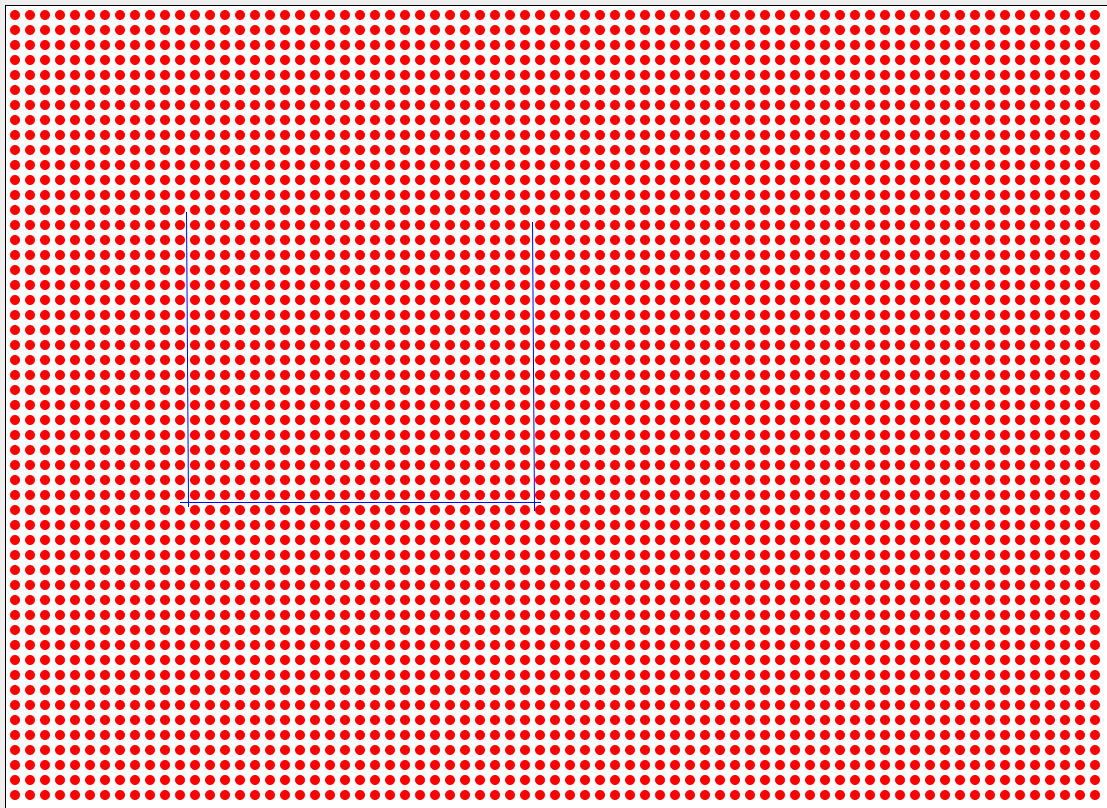
\includegraphics[scale=0.6]{cas_test.png}
\caption{Création du scénario de test de performances}
\end{figure}

Nous avons lancé l’exécution, puis l’avons mise en pause pour consulter les performances que nous avions eues.

\begin{figure}[H]
\centering
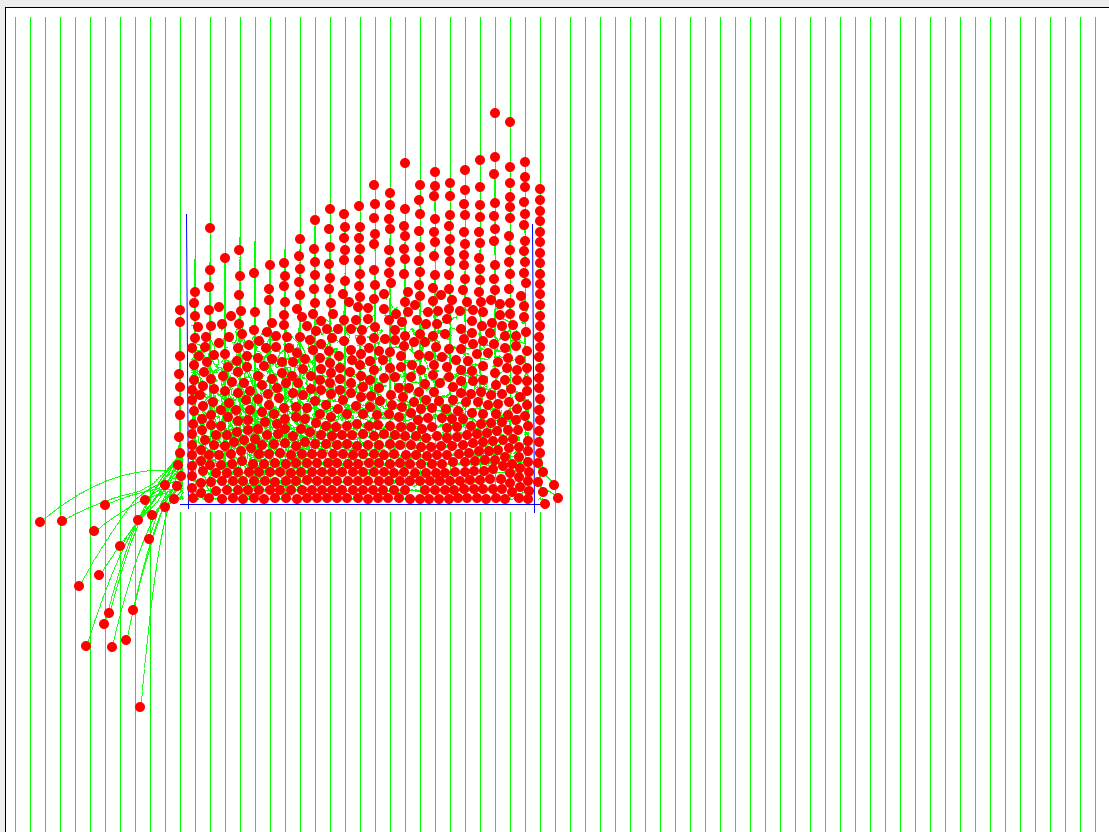
\includegraphics[scale=0.6]{one_time_tests.png}
\caption{Instant du scénario dont on mesure les performances}
\end{figure}

À cet instant, nous avons eu des déplacements de billes (certaines sont sorties de l’écran), des collisions bille-bille et des collisions bille-obstacle.

\newpage
Voici alors l’état de l’utilisation de notre machine : \\


\underline{Utilisation de la mémoire :}

\begin{figure}[H]
\centering
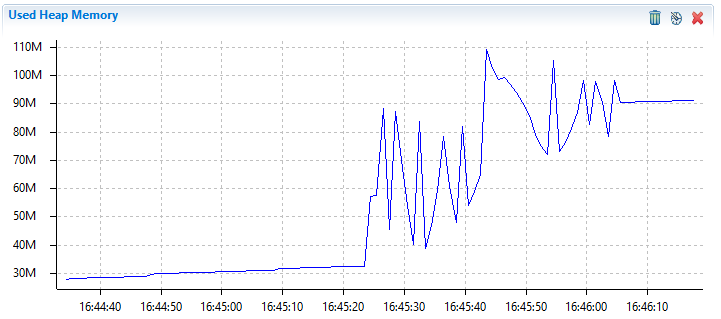
\includegraphics[scale=0.9]{timeline_memory.png}
\caption{Taux d'utilisation de la mémoire avec 4000 billes}
\end{figure}

Jusqu’à 16:45:25, notre application est “au repos” : on crée le circuit mais on ne fait aucune opération. Dans ce cas, notre application ne consomme que peu (entre 30 et 40Mo) de ressources. 

À 16:45:25, on lance la simulation et les 4000 billes se mettent alors à se déplacer et se rentrer dedans. L’exécution est mise en pause à 16:46:05.
Pendant ce laps de temps, on voit que notre application a consommé jusqu’à 110Mo de RAM. 
    
Ce qui nous intéresse ici est surtout de voir que dans un cas coûteux (avec 4000 billes), notre application n’utilise que 110Mo de RAM, ce qui est acceptable, la majorité des ordinateurs actuels possédant au minimum 1 ou 2 Go de RAM. \\

\newpage
\underline{Utilisation du CPU :}

\begin{figure}[H]
\centering
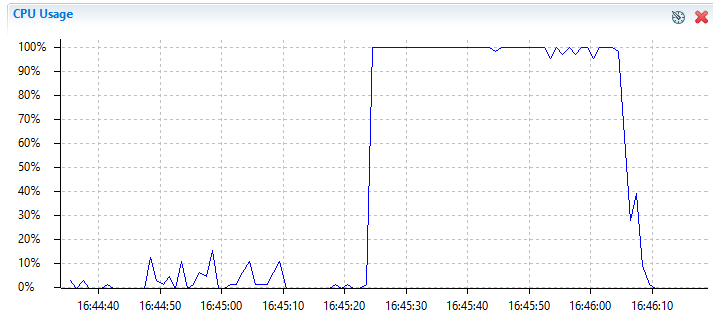
\includegraphics[scale=0.9]{timeline_cpu.png}
\caption{Taux d'utilisation du processeur avec 4000 billes}
\end{figure}

Au moment où la simulation est lancée via le bouton “Lancer” (vers 16:45:25), on voit que le CPU monte quasiment instantanément à 100\% d’utilisation. En effet, c’est à partir de ce moment que se lancent tous les calculs de vitesses, coordonnées, collisions et d’actualisation d’affichage. Le nombre de billes à cet instant est donc trop important pour faire fonctionner l’application de façon optimale.

Cependant, bien que beaucoup de billes sortent du circuit au cours de la simulation (elles ne sont donc plus prises en compte dans les méthodes de gestion de collisions et d’affichage), on voit que l’utilisation CPU reste quand même aux alentours de 100\% (entre 16:45:25 et 16:46:05 environ). On peut donc en déduire que le nombre de billes restant ralentit toujours notre application.

Enfin, une fois la simulation stoppée (vers 16:46:05), l’utilisation CPU retombe très vite à 0\% : tous les calculs de collisions et d’actualisation d’affichage s’arrêtent donc aussi, ce qui est le comportement prévu.

\newpage
Par ailleurs, nous avons effectué un test permettant de déterminer le pourcentage de CPU utilisé par méthode incluse dans l’application. Les résultats obtenus se trouvent sur l’image suivante :

\begin{figure}[H]
\centering
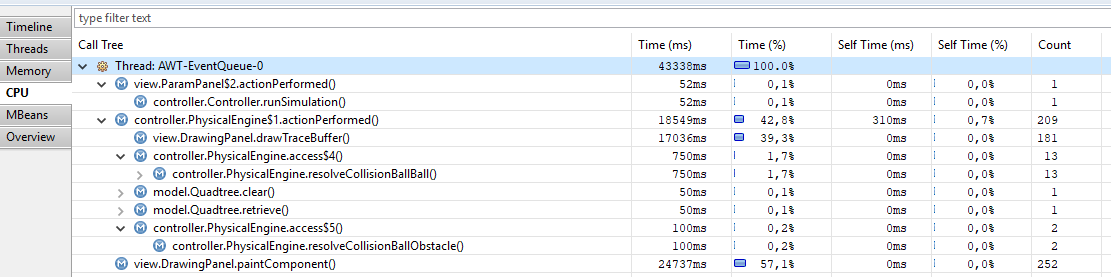
\includegraphics[scale=0.6]{CPU.png}
\caption{Utilisation du processeur par les méthodes avec 4000 billes}
\end{figure}

On peut voir qu’au cours d’une simulation, la majeure partie du processeur est utilisée par deux méthodes : \texttt{PhysicalEngine.actionPerformed} (une boucle d’exécution de la simulation dans la fonction \texttt{run()}) à hauteur de 42.8\%, et \texttt{DrawingPanel.paint} à hauteur de 57\%. Sachant que 39.3\% de l’utilisation de la méthode \texttt{PhysicalEngine.actionPerformed} est utilisée pour faire \texttt{DrawingPanel.drawTraceBuffer}, on a donc la mise à jour de l’affichage qui coûte 57.1\% + (42.8\% * 39.3\%) = 73.9\% du processeur.


\subsection{Avec 700 billes}

Nous avons continué à tester les performances de notre application (avec la même machine et le même circuit) tout en diminuant le nombre de billes au fur et à mesure, jusqu’à obtenir un cas d’utilisation qui est proche de la limite de vitesse optimale de fonctionnement de notre application. Le cas d’utilisation trouvé est donc avec environ 700 billes (764 exactement). \\

\underline{Utilisation de la mémoire : }

\begin{figure}[H]
\centering
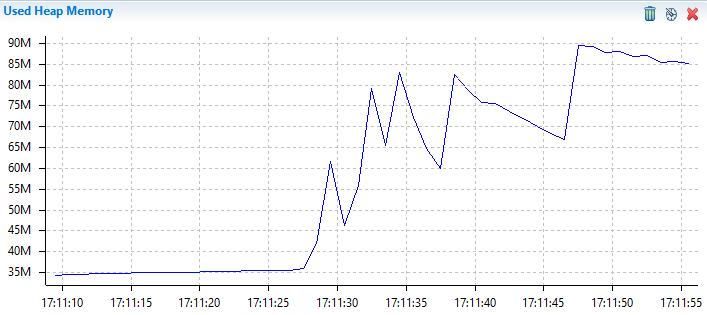
\includegraphics[scale=0.8]{timeline760_memory.png}
\caption{Taux d'utilisation de la mémoire avec 760 billes}
\end{figure}

Lors d’une exécution avec 760 billes, notre application atteint une consommation maximale de RAM de 90Mo. \\

\underline{Utilisation du CPU :}

\begin{figure}[H]
\centering
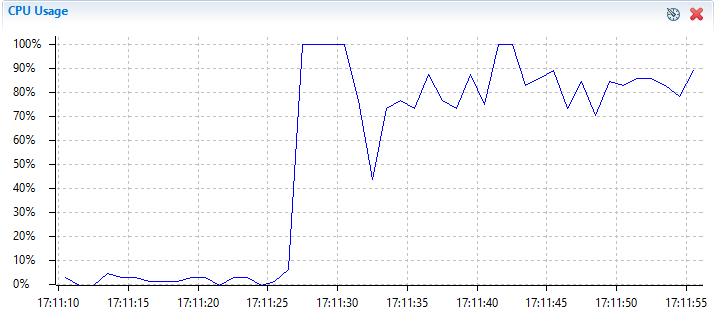
\includegraphics[scale=0.9]{timeline760_cpu.png}
\caption{Taux d'utilisation du processeur avec 760 billes}
\end{figure}

On remarque en effet que, sur la machine sur laquelle nous avons testé notre application, le processeur n’est pas utilisé à 100\% lors d’une simulation avec 760 billes.

\subsection{Tests avec et sans Quadtree}

L’utilisation du Quadtree réduit fortement le nombre de calculs à réaliser pour la détection de collisions. On passe d’une complexité en temps O(\(n^2\)) à une complexité de l’ordre de O(n log(n)). Voici deux tests qui vérifient ce gain de performances : \\

Nombre de billes : 3869\\

Nombre d’appels à \texttt{checkCollisionsBallBall} :
\begin{itemize}
\item sans Quadtree : 14 969 161
\item avec Quadtree : 476 070
\end{itemize}
On note une différence de facteur 30.

Nombre de billes : 104 411\\

Nombre d’appels à \texttt{checkCollisionsBallBall} :
\begin{itemize}
\item sans Quadtree : 10 901 656 921
\item avec Quadtree : 64 384 669
\end{itemize}
On note une différence de facteur 170.

\newpage
\section{Test de couverture}

Dans ce test, nous allons voir quelles fonctions (et quelles parties de fonctions) ont été atteintes lors de l’exécution du programme sur un scénario précis. L’objectif du test est de mettre en évidence le code “mort” dans notre application (code qui n’est jamais utilisé). L’idéal est donc d’avoir une couverture la plus large possible des fonctions appelées au cours d’un scénario.

Ici, nous avons créé deux obstacles, trois billes, modifié l’inclinaison du circuit, lancé la simulation et stoppé celle-ci. L’image ci-dessous montre l’état de l’application au moment où l’on a stoppé la simulation.


\begin{figure}[H]
\centering
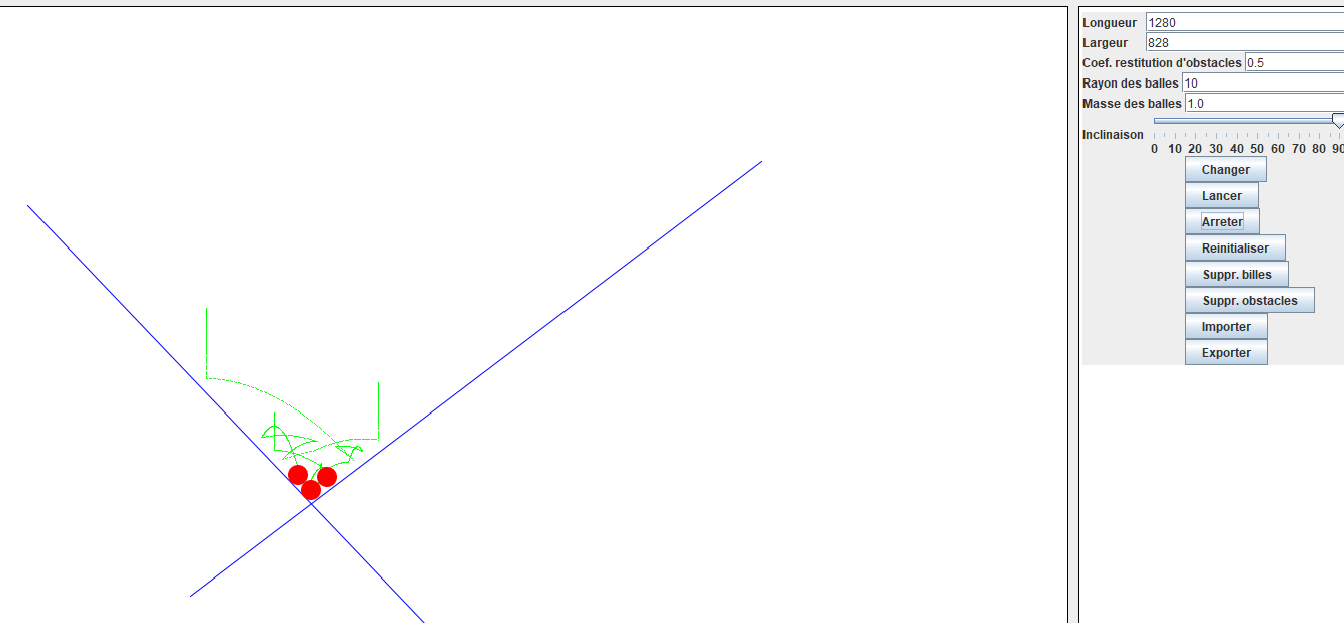
\includegraphics[scale=0.8]{cas_cov.png}
\caption{Scénario pour le test de couverture}
\end{figure}

Les fonctions de l’interface graphique n’étant appelées que si l’utilisateur génère un événement, ses tests de couverture sont nombreux puisqu’il faut tester plusieurs actions et combinaisons d’actions parmi toutes celles proposées par l’interface. 
Nous ne nous intéresserons donc qu’aux fonctions du moteur physique pour ce test de couverture.

\newpage
Les résultats du test sur cette exécution sont visibles sur l’image suivante :

\begin{figure}[H]
\centering
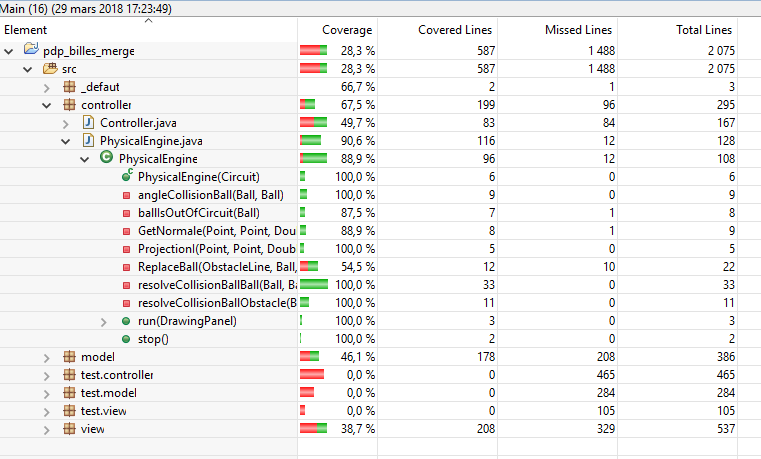
\includegraphics[scale=0.8]{coverage.png}
\caption{Couverture du programme sur un scénario}
\end{figure}

Dans notre cas d’utilisation, au cours de la simulation, les billes se sont déplacées, il y a eu des collisions billes-billes et des collisions billes-obstacle.

On peut voir que, dans la classe \texttt{PhysicalEngine}, 88.9\% du code est utilisé. En décomposant ses méthodes, on voit que c’est notamment la méthode \texttt{ReplaceBall} qui n’est utilisée qu’à moitié : cette méthode sert à repositionner correctement les billes dans le cas où, après un pas de temps, elles se superposent avec un obstacle.

Cependant, la méthode \texttt{ReplaceBall} n’utilise pas les mêmes bouts de code en fonction de l’angle ou du côté duquel elle arrive. Elle n’est donc pas entièrement atteinte dans notre cas d’utilisation.

Excepté cette méthode, la quasi-intégralité du moteur physique est utilisé. On peut donc estimer le test comme concluant.


%%% PARTIE 7 : EXTENSIONS %%%
\chapter{Extensions}

\section{Moteur physique}

\subsection{Frottements}

La simulation actuelle peut être considérée comme “dans le vide”, c’est-à-dire que seule la gravité influe sur le circuit. Il n’y a aucune perte d’énergie (sauf en cas de collision avec coefficient de rebond inférieur à 1). Dans le cas où on voudrait rendre le simulateur plus réaliste, il faudrait y rajouter la force de frottements. \\

Pour cela, il faudrait l'ajouter dans la méthode \texttt{step()} de la classe Ball, via un facteur qui modifierait l’accélération des billes selon leur taille et leur masse.

\subsection{Modifier la vitesse de la simulation}

Lors d’une simulation, la vitesse de la simulation est verrouillée. Cependant, il peut être intéressant de l’accélérer pour obtenir le résultat final plus rapidement, ou au contraire la ralentir pour mieux observer le parcours des billes à un certain moment. \\

Pour cela, on pourrait créer un slider (comme celui de l’inclinaison) afin de modifier en temps réel la vitesse de la simulation. Ce slider pourrait modifier la vitesse par un facteur compris entre 0.5 et 2.


\subsection{Retour à un temps antérieur de la simulation}

Notre application sauvegardant les traces des billes lors de la simulation, elle pourrait proposer une fonctionnalité de “retour dans le passé” pour rejouer la simulation à partir d’un instant précis. Il faudrait pour cela compter et actualiser la taille de la trace des billes au cours de la simulation. \\

A l’aide de l’interface graphique, on proposerait à l’utilisateur de choisir un entier i entre 0 et la taille de la trace des billes (qui est la même pour toutes les billes excepté pour celles qui sont sorties de l’écran puisqu’on ne les déplace plus) et on replacerait chaque bille à sa trace i et on effacerait toutes les traces après la i-ème.

\newpage
\subsection{Pas de temps évolutif}

Le pas de temps est actuellement modifiable à l’aide du panneau de paramétrage afin de choisir entre une simulation plus rapide mais moins précise, et une simulation fine mais lente. \\

Il pourrait être intéressant d’intégrer un pas de temps évolutif : lors de la simulation, on récupère à chaque pas de temps la vitesse la plus élevée d’une bille, et on adapte le pas de temps en fonction de cette vitesse. Ainsi, plus la bille est rapide, plus le pas de temps est diminué afin d’améliorer la précision de la simulation. La distance parcourue par une bille lors d’un pas de temps ne devrait jamais être supérieure à son rayon.

\section{Interface graphique}

\subsection{Déplacement d'un objet à la souris}

Actuellement, il faut cliquer droit sur un objet pour modifier ses coordonnées (x,y). Une amélioration possible est l’ajout d’un déplacement à la souris : en maintenant par exemple Ctrl + clic droit enfoncé sur un objet, on peut ensuite le faire glisser n’importe où sur le circuit pour le repositionner.

\subsection{Sélection de groupe d'objets}

Dans notre application, on ne peut interagir qu’avec un seul objet à la fois avec le clic droit. L’interface graphique peut être améliorée en ajoutant un système de sélection de groupe d’objets : en maintenant Ctrl + clic gauche enfoncé, on peut sélectionner un ensemble d’objets. Les objets sélectionnés pourront alors être déplacés simultanément à la souris, ou avoir un paramètre en commun modifié simultanément (exemple : la masse pour un groupe de billes).

\subsection{Zoom}

Pour améliorer la visibilité de notre circuit, surtout lorsqu’il y a beaucoup d’objets ou de petits objets, on pourrait implémenter un zoom à notre interface graphique. \\
=============
A l’aide de la molette de la souris, on appellerait une fonction qui modifierait un facteur de zoom. Chaque fois que ce facteur de zoom est modifié, il faudrait modifier l’échelle du panneau de dessin et des objets qui se trouvent dessus. \\

De plus, si on implémente un zoom centré sur la position de la souris au moment où l’événement “défilement molette” est appelé, il faut par la suite recalculer les coordonnées de la souris sur le circuit. En outre, lorsqu’on clique par exemple sur le coin en haut à gauche du panneau de dessin, quel que soit le facteur de zoom, les coordonnées de ce point sur le panneau seront (0,0). Or, si on a au préalable zoomé sur le coin en bas à gauche du circuit, on s’attend à avoir une autre valeur. \\

Il faut, à ce moment, bien faire la distinction entre le circuit et son affichage sur l’interface en corrigeant les coordonnées de la souris lorsqu’on a besoin d’utiliser ses coordonnées alors qu’on est en train de zoomer.

\newpage
\subsection{Couleur de billes unique}

Pour améliorer la lisibilité de notre application, on pourra créer un couple (bille, couleur) unique pour chaque bille de telle sorte que chaque bille soit d’une couleur différente et que la couleur de la trace d’une bille soit de la même couleur que celle-ci. De cette façon, lorsque plusieurs billes sont proches, on arrive à distinguer leurs traces les unes des autres. \\

Étant donné que notre application permet de gérer un nombre relativement grand de billes (quelques milliers), on pourra -répéter l’apparition de certaines couleurs. Il faut par contre éviter de proposer une palette de couleurs trop proches car cela rendrait leur distinction difficile ; et cela serait encore pire pour un daltonien. \\

Pour aller plus loin, on pourra laisser à l’utilisateur la possibilité de changer la couleur d’une bille dans sa fenêtre de paramétrage. Il faudra alors recolorier une autre bille afin de conserver un équilibre entre le nombre de billes par couleur


\subsection{Choix d'affichage des traces}

Il conviendrait de donner la possibilité à l’utilisateur d’afficher ou masquer la trace d’une ou plusieurs billes pendant l’exécution. Cela permettrait de pouvoir se concentrer sur le comportement de certaines billes parmi un grand nombre.

\section{Gestion du circuit}

\subsection{Billes - Coefficient de restitution}

Pour améliorer la paramétrabilité de notre application, on pourrait rendre modifiable le coefficient de restitution des billes. De la même manière que pour les obstacles, ce coefficient serait pris en compte lors d’une collision avec un autre objet du circuit et impacterait sur l’amplitude du rebond qui en découlerait.

\subsection{Obstacles - Formes}

L’application propose uniquement des obstacles sous forme de lignes individuelles. Nous pourrions ajouter plus de formes, comme des rectangles ou des cercles. \\

Pour cela, on ajouterait dans la barre de paramétrage des icônes permettant de sélectionner un objet à créer, et en fonction de l’objet sélectionné, un événement de clic du panneau de dessin associé à cet objet serait utilisé. Il faudrait alors les intégrer dans l’import/export. \\

De plus, il pourrait être possible de créer ses propres obstacles à l’aide d’un éditeur d’obstacles, où l’utilisateur peindrait à la souris son propre obstacle. Cependant, une forme quelconque est plus compliquée à gérer au niveau de la structure de données la représentant : il pourrait s’agir uniquement d’une liste de points. Cela rendrait l’export de cette forme beaucoup plus lourd que quelques attributs bien choisis. \\

Enfin, cette extension complexifierait notamment le moteur physique car, pour chaque nouveau type d'obstacle, il faudra gérer les collisions (détection et résolution) de manières différentes.


\section{Gestion de fichiers}

\subsection{Vidéo de l'exécution}

Nous pourrions ajouter à notre application la possibilité d’enregistrer le panneau de dessin. Il faudrait pour cela ajouter un bouton permettant au premier clic de débuter un enregistrement et au second de terminer l’enregistrement et d’ouvrir une interface de gestion de fichier pour la sauvegarde de la vidéo. \\

Pour réaliser l’enregistrement en lui-même, on pourrait :
\begin{itemize}
\item utiliser une bibliothèque capable d’enregistrer ce qui se passe sur le panneau de dessin. Cette méthode permet de n’enregistrer que ce qui nous intéresse, mais nécessite sans doute une compatibilité de la bibliothèque d’enregistrement avec notre bibliothèque d’affichage SWING.
\item utiliser une bibliothèque capable d’enregistrer ce qui se passe sur la fenêtre de l’application. Avec cette méthode, il y a moins de risques de compatibilité avec la bibliothèque d’affichage. En revanche, on ne capture pas que la simulation.
\end{itemize}




\subsection{Amélioration de l'import}

\subsubsection{Changement d'échelle à l'import}

Actuellement, lors de l’import d’un circuit dans l’application, si la taille de l’écran de l’utilisateur ne permet  pas d’afficher le circuit importé en entier, le circuit importé est rogné à la taille maximale possible sur l’écran de l’utilisateur. Une amélioration de notre application serait alors de permettre à ce genre d’import de ne pas être rogné en changeant l’échelle d’affichage du circuit. Cela équivaut à “zoomer en arrière” et peut donc se coupler avec l’extension “Zoom”.

\subsubsection{Fusion de circuits}

Dans notre application, lorsqu’on importe un circuit, on efface systématiquement celui qui était présent avant. Il est donc possible d’améliorer notre logiciel en permettant la fusion de circuits : c’est-à-dire que lorsqu’on importe un circuit, on a la possibilité de le “coller” à côté du circuit déjà présent. Ces deux circuits seraient alors fusionnés pour n’en faire qu’un, leur inclinaison devenant liée. Lorsque deux circuits fusionnent, il faut alors permettre à une bille de s’écouler de l’un à l’autre. En outre, on peut imaginer qu’on avait deux circuits en carton et que nous les avons mis côte-à-côte sur un bord. \\

\newpage
On peut imaginer qu’on puisse ensuite à nouveau fusionner un circuit à notre circuit composé, et ainsi permettre la fusion entre plusieurs circuits.
Cette fonctionnalité nécessiterait de mettre en place un “mode fusion” dans lequel on verrait nos deux circuits (celui déjà présent et celui que l’on souhaite importer) et permettrait de choisir le côté sur lequel on va fusionner les deux circuits. \\

Pour cela, on pourra définir une position par défaut du circuit à fusionner sur le circuit existant, puis proposer à l'utilisateur de faire glisser ce premier autour de ce dernier en faisant une translation des coordonnées du circuit "mobile", en fonction des actions de l'utilisateur. \\

Sur la figure ci-dessous, en noir figure le circuit déjà présent et en rouge, des possibilités de fusions  :

\begin{figure}[H]
\centering
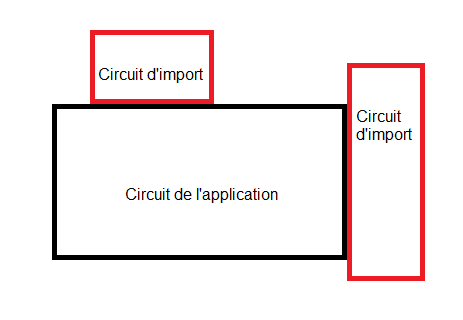
\includegraphics[scale=1.0]{fusioncircuits.png}
\caption{Schéma de possibilité de fusion de circuits}
\end{figure}

%%% PARTIE 8 : CONCLUSION %%%
\chapter{Conclusion}

Dans le cadre de ce projet, nous avons été amenées à étudier plusieurs lois physiques telles que la mécanique du point avec le mouvement rectiligne uniformément accéléré, ainsi que les chocs élastiques et inélastiques. Ces recherches nous ont permis de concevoir un moteur physique tentant de correspondre le plus possible à la réalité. Bien qu’essentielles, nous nous sommes rendus compte à quel point les recherches et la compréhension d’un domaine éloigné du nôtre pouvaient êtres coûteuses en temps. \\

Toutefois, nous pensons avoir atteint les objectifs du projet, bien que ceux-ci aient été ambitieux. Notre logiciel, malgré ses limites, permet la création, la personnalisation, l’import et l’export de circuits à travers une interface homme-machine que nous jugeons assez simple pour être comprise par n’importe quel utilisateur familier des écoulements de billes, bien que son ergonomie reste discutable. \\

Le moteur physique, quant à lui, permet de simuler un lâché de billes sur un plan incliné et parsemé d’obstacles. Les résolutions de collisions sont pour la majorité correctement calculées, ce qui permet d’avoir un moteur physique respectant la physique, au moins en apparence.
En revanche, notre moteur ne possédant pas de frottements, notre application ne peut être assimilée à un simulateur d’écoulements de billes soumis aux lois de la physique terrestre. \\

Notre application est évolutive et pourrait être améliorée et étendue, par exemple en implémentant les frottements, en corrigeant les bugs restants, et en implémentant de nouvelles fonctionnalités.

\bibliographystyle{unsrt}
\bibliography{biblio.bib}

\end{document}
